\documentclass[11pt,letterpaper]{article}

\addtolength{\oddsidemargin}{-.875in}
\addtolength{\evensidemargin}{-.875in}
\addtolength{\textwidth}{1.75in}

\addtolength{\topmargin}{-.875in}
\addtolength{\textheight}{1.75in}

\usepackage[utf8]{inputenc}
\usepackage{caption} % for table captions
\usepackage{amsmath} % for multi-line equations and piecewises
\DeclareMathOperator{\sign}{sign}
\usepackage{graphicx}
\usepackage{relsize}
\usepackage{xspace}
\usepackage{verbatim} % for block comments
\usepackage{subcaption} % for subfigures
\usepackage{enumitem} % for a) b) c) lists
\newcommand{\Cyclus}{\textsc{Cyclus}\xspace}%
\newcommand{\Cycamore}{\textsc{Cycamore}\xspace}%
\newcommand{\deploy}{\texttt{d3ploy}\xspace}%
\newcommand{\Deploy}{\texttt{D3ploy}\xspace}%
\usepackage{tabularx}
\usepackage{color}
\usepackage{multirow}
\usepackage{float}
\usepackage[acronym,toc]{glossaries}
\newacronym{ANL}{ANL}{Argonne National Laboratory}
\newacronym{B4C}{B4C}{boron carbide}
\newacronym{BC}{BC}{boundary condition}
\newacronym{BOC}{BOC}{beginning of equilibrium cycle}
\newacronym{BSD}{BSD}{Berkeley Software Distribution}
\newacronym{BWR}{BWR}{Boiling Water Reactor}
\newacronym{CAISO}{CAISO}{California ISO}
\newacronym{CEA}{CEA}{Commissariat a l'Energie Atomique}
\newacronym{CFD}{CFD}{computational fluid dynamics}
\newacronym{CO2}{CO$_2$}{carbon dioxide}
\newacronym{CR}{CR}{control rod}
\newacronym{CRP}{CRP}{Coordinated Research Project}
\newacronym{CZP}{CZP}{Cold Zero Power}
\newacronym{DCC}{DCC}{depressurized conduction cool-down}
\newacronym{DOE}{DOE}{Department of Energy}
\newacronym[\glslongpluralkey={degrees of freedom}]{DoF}{DoF}{degree of freedom}
\newacronym{EOC}{EOEC}{end of equilibrium cycle}
\newacronym{FCEV}{FCEV}{Fuel Cell Electric Vehicle}
\newacronym{FDM}{FDM}{Finite Difference Method}
\newacronym{FEM}{FEM}{Finite Element Method}
\newacronym{FVM}{FVM}{Finite Volume Method}
\newacronym{FSV}{FSV}{Fort St. Vrain}
\newacronym[\glslongpluralkey={greenhouse gases}]{GHG}{GHG}{greenhouse gas}
\newacronym{GRS}{GRS}{Gesellschaft für Anlagen und Reaktorsicherheit}
\newacronym{H2}{H$_2$}{hydrogen}
\newacronym{He}{He}{helium}
\newacronym{HFP}{HFP}{Hot Full Power}
\newacronym{HPCC}{HPCC}{high pressure conduction cool-down}
\newacronym{HTE}{HTE}{High-Temperature Electrolysis}
\newacronym{HTGR}{HTGR}{High-Temperature Gas-Cooled Reactor}
\newacronym{HTR}{HTR}{High Temperature Reactor}
\newacronym{HTTR}{HTTR}{High Temperature Test Reactor}
\newacronym{HZDR}{HZDR}{Helmholtz-Zentrum Dresden-Rossendorf}
\newacronym{IAEA}{IAEA}{International Atomic Energy Agency}
\newacronym{icap}{iCAP}{Illinois Climate Action Plan}
\newacronym{INL}{INL}{Idaho National Laboratory}
\newacronym{IPyC}{IPyC}{inner pyrolytic carbon}
\newacronym{JFNK}{JFNK}{Jacobian-Free Newton-Krylov}
\newacronym{KAERI}{KAERI}{Korea Atomic Energy Research Institute}
\newacronym{Keff}{K$_{eff}$}{multiplication factor}
\newacronym{LBP}{LBP}{Lumped Burnable Poison}
\newacronym{LGPL}{LGPL}{Lesser GNU Public License}
\newacronym{LOCA}{LOCA}{loss of coolant accident}
\newacronym{LPCC}{LPCC}{low pressure conduction cool-down}
\newacronym{LTE}{LTE}{Low-Temperature Electrolysis}
\newacronym{LWR}{LWR}{Light Water Reactor}
\newacronym{MC}{MC}{Monte Carlo}
\newacronym{MHTGR}{MHTGR}{Modular High-Temperature Gas-Cooled Reactor}
\newacronym{MOC}{MOC}{middle of equilibrium cycle}
\newacronym{MOOSE}{MOOSE}{Multi-physics Object-Oriented Simulation Environment}
\newacronym{MPI}{MPI}{Message Passing Interface}
\newacronym{MSR}{MSR}{Molten Salt Reactor}
\newacronym{MTD}{MTD}{Champaign-Urbana Mass Transit District}
\newacronym{NEA}{NEA}{Nuclear Energy Agency}
\newacronym{NEM}{NEM}{Nodal Expansion Method}
\newacronym{NGNP}{NGNP}{Next Generation Nuclear Power}
\newacronym{NRC}{NRC}{Nuclear Regulatory Commission}
\newacronym{NSC}{NSC}{Nuclear Science Committee}
\newacronym{OECD}{OECD}{Organisation for Economic Co-operation and Development}
\newacronym{OPyC}{OPyC}{outer pyrolytic carbon}
\newacronym{ORNL}{ORNL}{Oak Ridge National Laboratory}
\newacronym{OS}{OS}{Operator-Splitting}
\newacronym{PBMR}{PBMR}{Pebble Bed Modular Reactor}
\newacronym{PDE}{PDE}{Partial Differential Equation}
\newacronym{PMR}{PMR}{Prismatic Modular Reactor}
\newacronym{PV}{PV}{photovoltaics}
\newacronym{RSC}{RSC}{Reserve Shutdown Control}
\newacronym{RSD}{RSD}{Relative Standard Deviation}
\newacronym{SD}{SD}{Standard Deviation}
\newacronym{SI}{SI}{Sulfur-Iodine}
\newacronym{SiC}{SiC}{silicon carbide}
\newacronym{SMR}{SMR}{Small Modular Reactor}
\newacronym{SNU}{SNU}{Seoul National University}
\newacronym{SOEC}{SOEC}{Solid Oxide Electrolysis Cells}
\newacronym{TIP}{TIP}{transverse integration procedure}
\newacronym{TRISO}{TRISO}{Tristructural Isotropic}
\newacronym{UIUC}{UIUC}{University of Illinois at Urbana-Champaign}
\newacronym{UNIST}{UNIST}{Ulsan National Institute of Science and Technology}
\newacronym{UK}{UK}{United Kingdom}
\newacronym{UMICH}{UMICH}{University of Michigan}
\newacronym{US}{US}{United States}
\newacronym{VHTR}{VHTR}{Very High Temperature Gas Cooled Reactor}
%\newacronym{<++>}{<++>}{<++>}
%\newacronym{<++>}{<++>}{<++>}

\definecolor{bg}{rgb}{0.95,0.95,0.95}
\newcolumntype{b}{X}
\newcolumntype{f}{>{\hsize=.15\hsize}X}
\newcolumntype{s}{>{\hsize=.5\hsize}X}
\newcolumntype{m}{>{\hsize=.75\hsize}X}
\newcolumntype{r}{>{\hsize=1.1\hsize}X}
\usepackage{titling}
\usepackage[hang,flushmargin]{footmisc}
\renewcommand*\footnoterule{}
\usepackage{tikz}

\usetikzlibrary{shapes.geometric,arrows}
\tikzstyle{process} = [rectangle, rounded corners,
minimum width=1cm, minimum height=1cm,text centered, draw=black,
fill=blue!30]
\tikzstyle{arrow} = [thick,->,>=stealth]

\graphicspath{}

\begin{document}

% Introduction or Objectives
% Efficient hydrogen production by \glspl{HTGR} motivates the last chapter of the thesis.
% We analyze several hydrogen production methods coupled to different nuclear reactor desings.
% In order to find the most efficient method, we not only consider \glspl{HTGR} but also other type of reactors.

\section{Introduction}

% The energy problem
Energy is one of the most vital contributors to economic growth.
In the future, economies will continue to expand, populations will do so too, and their energy demand will accompany such change \cite{burke_impact_2018} \cite{el-shafie_hydrogen_2019}.
Meeting these future needs requires the development of clean energy sources as environmental concerns continue to rise.

As seen in Figure \ref{fig:ghg}, electricity generation was one of the economic sectors that released the most \glspl{GHG} in the \gls{US} in 2017.
As \gls{CO2} is the main component in \glspl{GHG}, decarbonizing electricity generation will allow us to meet the increases in energy demand and address the environmental concerns simultaneously.

\begin{figure}[htbp!]
	\centering
	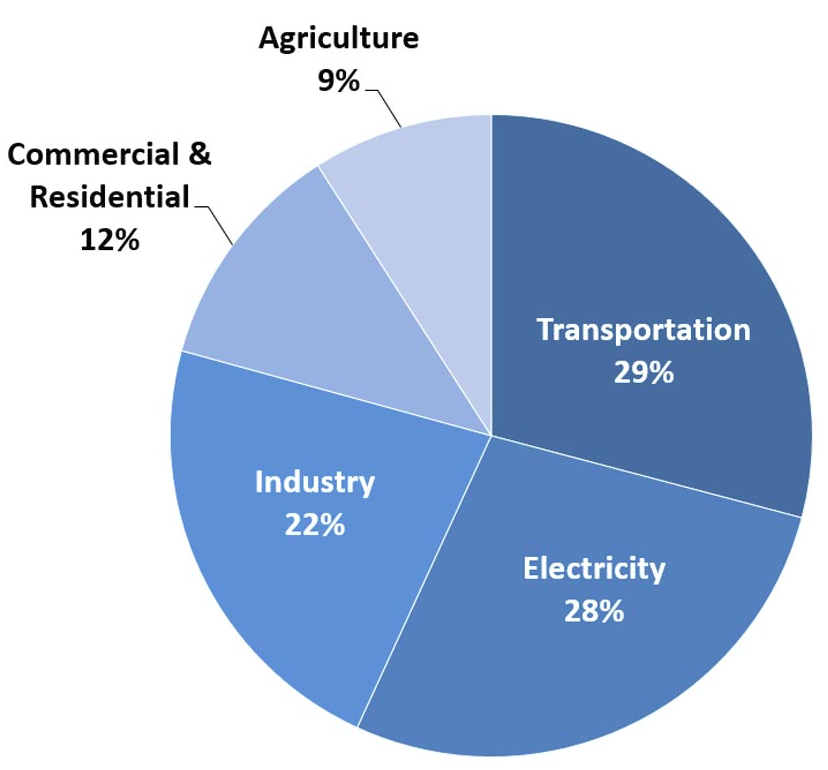
\includegraphics[width=0.4\linewidth]{figures-hydro /total-ghg-2017.png}
	\hfill
	\caption{Total \gls{US} \gls{GHG} emissions by economic sector in 2017. Image reproduced from \cite{us_epa_sources_2020}.}
	\label{fig:ghg}
\end{figure}

% word on solar energy and the duck curve
To address these concerns, utility companies are relying more and more on renewable energy resources, such as wind and solar \cite{ming_resource_2019}.
However, high solar adoption creates a challenge.
The need for electricity generators to quickly ramp up increases when the sun sets and the contribution from the \gls{PV} falls \cite{us_department_of_energy_confronting_2017}.
The "duck curve" (or duct chart) depicts this phenomenon, Figure \ref{fig:duck}.
The \gls{CAISO} developed the duck curve to illustrate the grid's net load \cite{bouillon_prepared_2014}.
We define the net load as the difference between forecasted load and expected electricity production from solar.

Moreover, the duck curve reveals another issue.
Over-generation may occur during the middle of the day, and high-levels of non-dispatchable generation may exacerbate the situation.
As a consequence, the market would experience sustained zero or negative prices during the middle of the operating day \cite{bouillon_prepared_2014}.

\begin{figure}[htbp!]
	\centering
	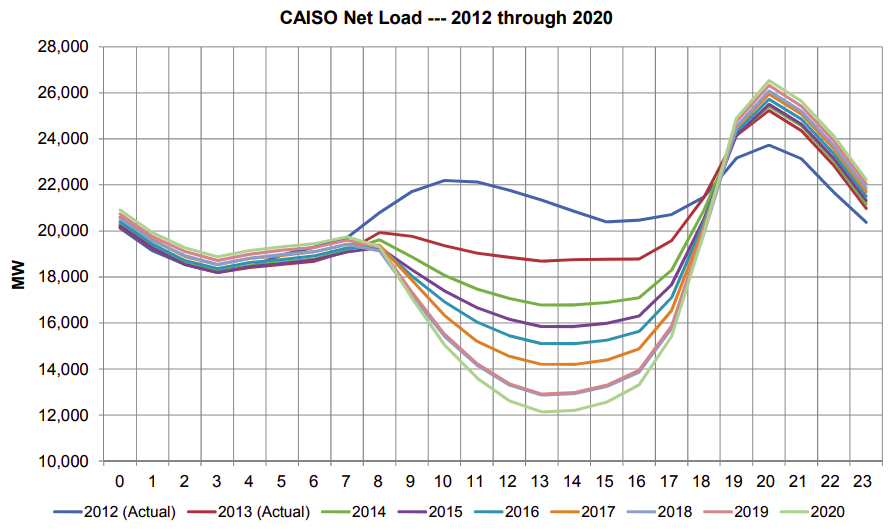
\includegraphics[width=0.75\linewidth]{figures-hydro /caiso-duck.png}
	\hfill
	\caption{The duck curve. Image reproduced from \cite{bouillon_prepared_2014}.}
	\label{fig:duck}
\end{figure}

% solutions to the duck curve
The simplest solution to a demand ramp-up is to increase dispatchable generation, resources with fast ramping and fast starting capabilities such as natural gas and coal \cite{bouillon_prepared_2014}, and, consequently, decrease non-dispatchable generation, such as geothermal, nuclear, and hydro.
Nonetheless, an approach like this is not consistent with the goal of reducing carbon emissions.
Hence, our focus drifts to other potential low-carbon solutions, like nuclear generation and electricity storage through \gls{H2} production.

% Transportation problem
Unfortunately, a carbon-neutral electric grid will be insufficient to halt climate change because transportation is a significant contributor to \gls{GHG} emissions.
As seen in Figure \ref{fig:ghg}, transportation released the most \glspl{GHG} in the \gls{US} in 2017. Thus, decarbonizing transportation underpins global carbon reduction.
One possible strategy is to develop a hydrogen economy, as Japan is currently doing.
Japan's strategy rests on the firm belief that \gls{H2} can be a decisive response to its energy and climate challenges.
It could foster deep decarbonization of the transport, power, industry, and residential sectors while strengthening energy security \cite{nagashima_japans_2018}.
In the transportation sector, Japan plans to deploy fuel cell vehicles, trucks, buses, trains, and ships.

Although \gls{H2} technologies do not release CO$_2$, any \gls{H2} production method is only as carbon-free as the energy source it relies on (electric, heat, or both).
Nuclear reactors introduce a clean energy option to manufacture \gls{H2}.

The \gls{UIUC} is leading by example and actively working to reduce \gls{GHG} emissions from electricity generation and transportation (among other sectors) on its campus.
In pursuance of those efforts, the university has developed the \gls{icap}.

\section{\gls{icap}}
% ICAPP
In 2008, \gls{UIUC} signed the American College and University Presidents' Climate Commitment, formally committing to becoming carbon neutral as soon as possible, no later than 2050.
The university developed the first \gls{icap} in 2010 as a comprehensive roadmap toward a sustainable campus environment \cite{university_of_illinois_at_urbana-champaign_illlinois_2015}.
The \gls{icap} defines a list of goals, objectives, and potential strategies for six topical areas.

\begin{itemize}
	\item Energy Conservation and Building Standards:
\end{itemize}
Focuses on maintaining or reducing campus gross square footage, strengthen conservation efforts, and engage the campus community in energy conservation.

\begin{itemize}
	\item Energy Generation, Purchasing, and Distribution:
\end{itemize}
Efforts towards the exploration of 100\% clean campus energy options.
This includes expanding on-campus solar energy production, the extension of the purchase of clean energy from low-carbon energy sources, and the offset of all emissions from the National Petascale Computing Facility.

\begin{itemize}
	\item Transportation:
\end{itemize}
This area comprises the efforts to reduce air travel emissions, reduce Urbana-Champaign campus fleet emissions, and study scenarios for complete conversion of the campus fleet to renewable fuels.

\begin{itemize}
	\item Water and Stormwater:
\end{itemize}
This area focuses on improving the water efficiency of cooling towers, perform a water audit to establish water conservation targets, determine upper limits for water demand by end-use, and implement projects to showcase the potential of water and stormwater reuse.

\begin{itemize}
	\item Purchasing, Waste, and Recycling:
\end{itemize}
Attempt to standardize office paper purchases, cleaning products, computers, other electronics, and freight delivery services.
It also attempts to foment recycling by reducing non-durable goods purchases and reducing municipal solid waste going to landfills.

\begin{itemize}
	\item Agriculture, Land Use, Food, and Sequestration:
\end{itemize}
This area will perform a comprehensive assessment of \gls{GHG} emissions from agricultural operations, and develop a plan to reduce them, implement a project that examines the foodservice carbon footprint for Dining, and increase carbon sequestration in campus soils.

\section{Objectives}

As mentioned earlier, we place our attention on two areas: electricity generation and transportation.
We will turn our attention to electricity generation and transportation on the \gls{UIUC} campus.
Consequently, this work's objective aligns with the efforts in two of the six target areas defined on the \gls{icap}.

Regarding electricity generation, our analysis focuses on the \gls{UIUC} grid.
The present work quantifies the magnitude of the duck curve in such a grid.
To mitigate the risk of over-generation, we propose to use the over-generated energy to manufacture \gls{H2}.
We chose a nuclear reactor to be the primary source of energy.
The next step is to quantify how much \gls{H2} different production methods can produce.
Section \ref{sec:hydro} discusses a few hydrogen production methods considered for our analysis.
Finally, we will calculate how much electricity we would generate using the \gls{H2} produced.

Regarding transportation, we study the conversion of the \gls{UIUC} fleet on campus to \glspl{FCEV}.
Additionally, the analysis includes the conversion of the \gls{MTD} fleet as well.
The first step is to determine the fuel consumed by both fleets and how much \gls{H2} enables the fleets' complete conversion.
Finally, we consider a few reactor designs and analyze which of them could produce enough \gls{H2} to fulfill both fleet requirements.

Both studies propose the same solution, a nuclear reactor coupled to a hydrogen plant.
In terms of electricity generation, this solution will decrease the need for dispatchable sources and, consequently, reduce carbon emissions.
In terms of transportation, it will eliminate carbon emissions.

%Mention the choice of reactor
In both analyses, many reactor choices can satisfy our needs.
The typical \gls{UIUC}'s grid demand is smaller than 80 MW \cite{dotson_optimal_2020}.
Accordingly, we consider reactors of small capacities, such as microreactors and \glspl{SMR}.
Section \ref{sec:reactors} discusses their characteristics.

\section{Hydrogen production methods}
\label{sec:hydro}

This section introduces several hydrogen production processes and their energy requirements.

\subsection{Electrolysis}

The electrolysis of water is a well-known method whose commercial use began in 1890.
This process produces approximately 4\% of \gls{H2} worldwide.
The process is ecologically clean because it does not emit \glspl{GHG}.
However, in comparison with other methods, electrolysis is a highly energy-demanding technology \cite{kalamaras_hydrogen_2013}.

Three electrolysis technologies exist.
Alkaline-based is the most common, the most developed, and the lowest in capital cost.
It has the lowest efficiency and, therefore, the highest electrical energy cost.
Proton exchange membrane electrolyzers are more efficient but more expensive than Alkaline electrolyzers.
\gls{SOEC} electrolyzers are the most electrically efficient but the least developed.
\gls{SOEC} technology has challenges with corrosion, seals, thermal cycling, and chrome migration \cite{kalamaras_hydrogen_2013}.
As the first two technologies work with liquid water and the latter requires high-temperature steam, we will refer to the first two as \gls{LTE} and the latter as \gls{HTE}.

Water electrolysis converts electric and thermal energy into chemical energy stored in hydrogen.
The process enthalpy change $\Delta H$ determines the required energy for the electrolysis reaction to take place.
Part of the energy corresponds to electric energy $\Delta G$ and its rest to thermal energy $T \cdot \Delta S$, Equation \ref{eq:electrolysis1}.

\begin{align}
	\Delta H &= \Delta G + T \Delta S
\label{eq:electrolysis1}
    \intertext{where}
    \Delta H &= \mbox{Total specific energy [kWh/kg-H$_2$]} \\
    \Delta G &= \mbox{Specific electrical energy [kWh/kg-H$_2$]} \\
    T \Delta S &= \mbox{Specific thermal energy [kWh/kg-H$_2$].}
\end{align}

In \gls{LTE}, electricity generates thermal energy.
Hence, $\Delta H$ alone determines the process required energy.
$\Delta H$ is equal to 60 kWh/kg-H$_2$ considering a 67$\%$ efficiency \cite{usdrive_hydrogen_2017}.

In \gls{HTE}, a high-temperature heat source is necessary to provide thermal energy.
$\Delta G$ decreases with increasing temperature, Figure \ref{fig:electro1}.
Decreasing the electricity requirement results in higher overall production efficiencies since heat-engine-based electrical work has a thermal efficiency of 50$\%$ or less \cite{j_e_obrien_high_2010}.
Figure \ref{fig:electro1} shows $\Delta G$ and $T \Delta$S.
$\Delta G$ considers the \gls{SOEC} to have an electrical efficiency of 88$\%$ \cite{helmeth_high_2020}.
$T \Delta S$ accounts for the latent heat of water vaporization.
Note that the process is at 3.5 MPa.
$\Delta G$ increases with pressure.
However, we chose a high pressure to save energy, as compressing liquid water is cheaper than compressing the hydrogen \cite{obrien_status_2019}.

\begin{figure}[htbp!]
	\centering
	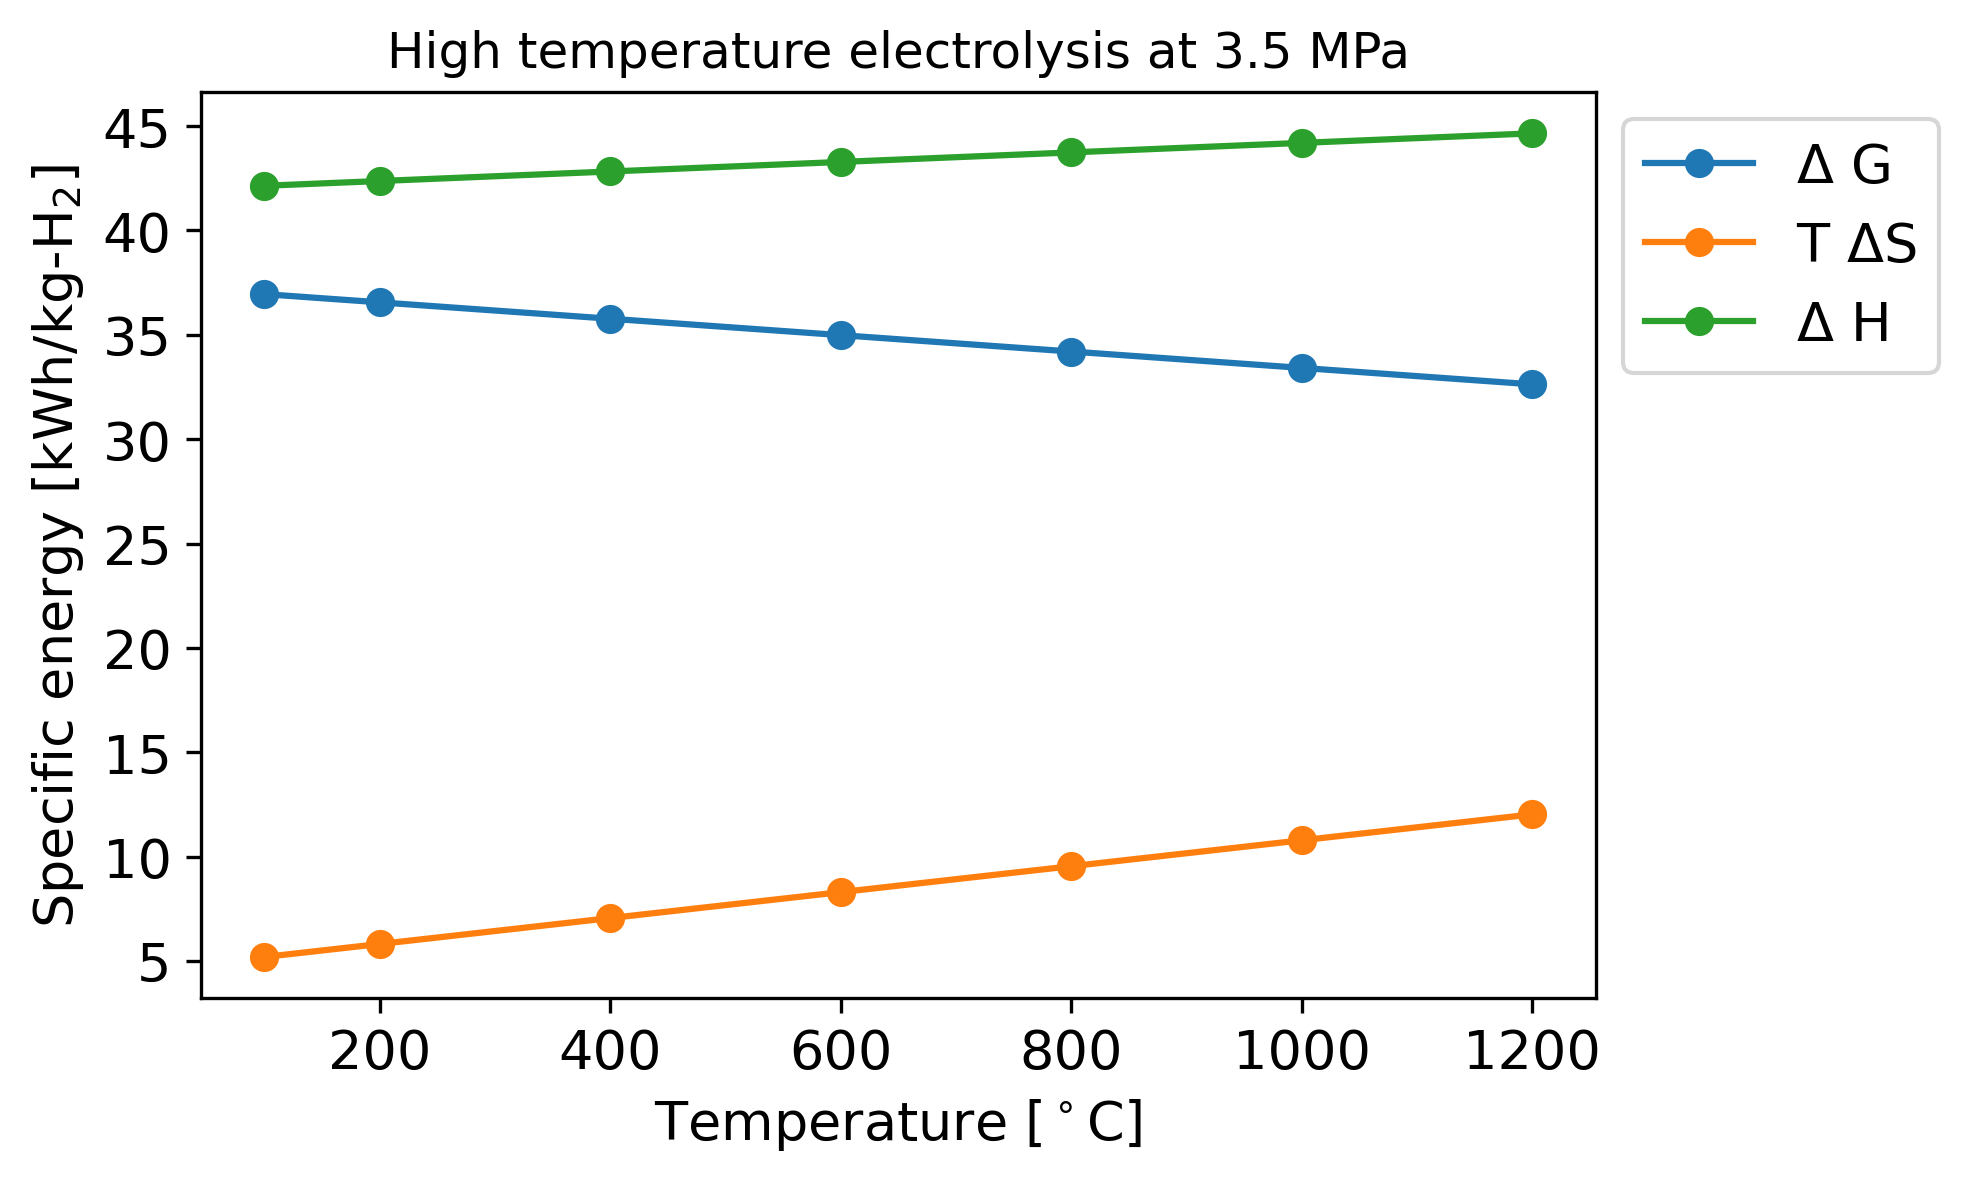
\includegraphics[width=0.8\linewidth]{figures-hydro /hte-energy-P.png}
	\hfill
	\caption{Energy required by \gls{HTE} at 3.5 MPa.}
	\label{fig:electro1}
\end{figure}

Finally, equations \ref{eq:electrolysis2a} and \ref{eq:electrolysis2b} determine the electrical $P_{EH2}$ and thermal power $P_{TH2}$ required by the hydrogen plant.

\begin{align}
	P_{EH2} &= \dot{m}_{H2} \Delta G \label{eq:electrolysis2a} \\
	P_{TH2} &= \dot{m}_{H2} T \Delta S \label{eq:electrolysis2b}
	\intertext{where}
	P_{EH2} &= \mbox{Total electrical power [kW]} \\
	P_{TH2} &= \mbox{Total thermal power [kW]} \\
	\dot{m}_{H2} &= \mbox{\gls{H2} production rate [kg/h].}
\end{align}

\subsection{Sulfur-Iodine Thermochemical Cycle}

Thermochemical water-splitting is converting water into hydrogen and oxygen by a series of thermally driven chemical reactions.
The direct thermolysis of water requires temperatures above 2500 $^{\circ}$C for significant hydrogen generation.
At this temperature, the process can decompose a 10\% of the water.
A thermochemical water-splitting cycle accomplishes the same overall result using much lower temperatures.

General Atomics, Sandia National Laboratories, and the University of Kentucky compared 115 cycles that would use high-temperature heat from an advanced nuclear reactor \cite{brown_high_2003}.
The report specifies a set of screening criteria used to rate each cycle.
The highest scoring method was the \gls{SI} Cycle.

The \gls{SI} cycle consists of the three chemical reactions represented in Figure \ref{fig:sulfur1}.
The whole process takes in water and high-temperature heat and releases hydrogen and oxygen.
The process does not use any electricity.
The process recycles all reagents and does not have any effluents \cite{yildiz_efficiency_2006}.
The chemical reactions are:

\begin{align}
	I_2 + SO_2 + 2H_2O &\rightarrow 2HI + H_2SO_4 \\
	H_2SO4 &\rightarrow SO_2 + H_2O + 1/2O_2 \\
	2HI &\rightarrow I_2 + H_2.
\end{align}

\begin{figure}[htbp!]
	\centering
	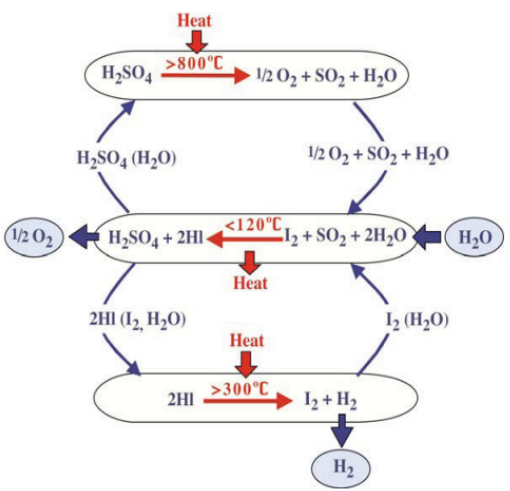
\includegraphics[width=0.5\linewidth]{figures-hydro /sulfur1.png}
	\hfill
	\caption{Diagram of the Sulfur-Iodine Thermochemical process. Image reproduced from \cite{benjamin_russ_sulfur_2009}.}
	\label{fig:sulfur1}
\end{figure}

Figure \ref{fig:sulfur2} presents the specific energy requirements of the cycle $\Delta H$.
Several sources disagree on the minimum temperature for the process to be viable.
Our analysis considers the process feasible only for temperatures above 800 $^{\circ}$C.
Finally, equation \ref{eq:sulfur4} determines the thermal power $P_{TH2}$ required by the hydrogen plant.

\begin{figure}[htbp!]
	\centering
	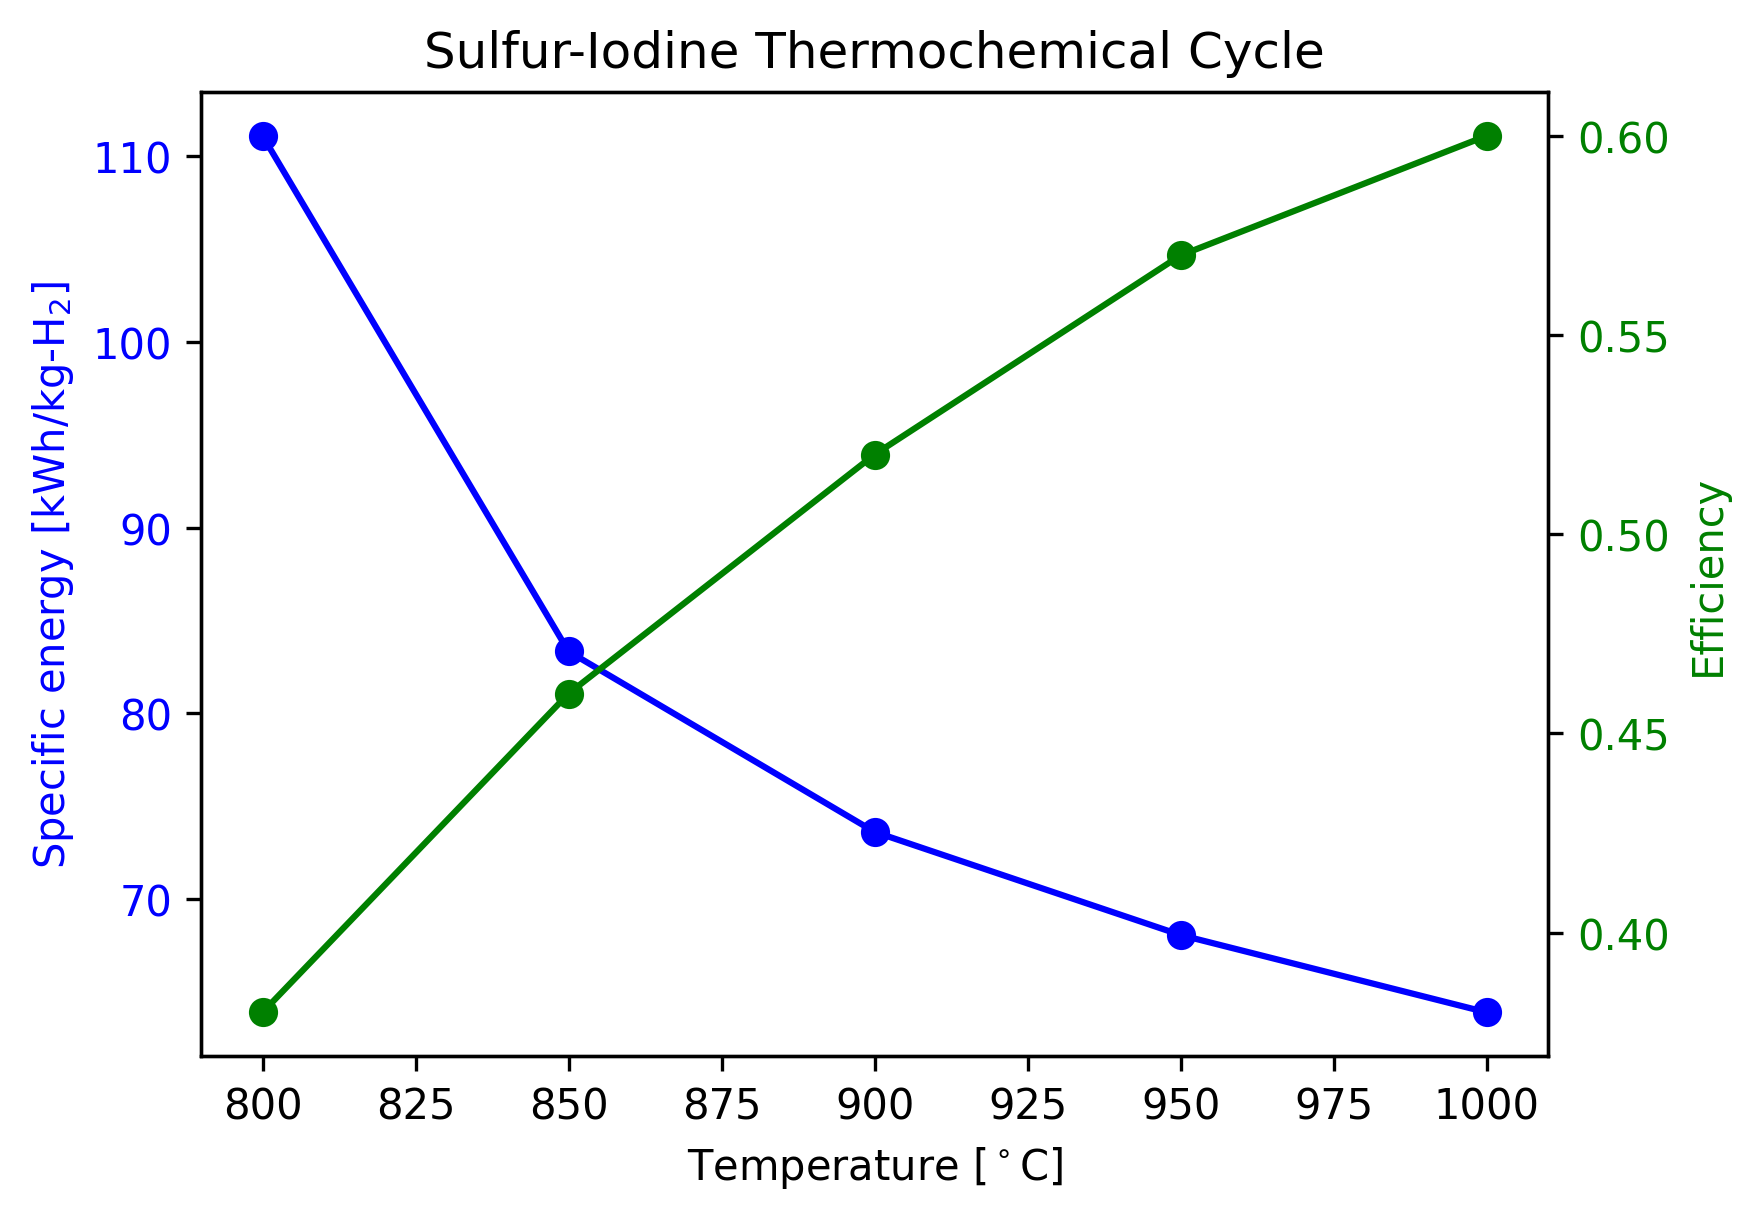
\includegraphics[width=0.7\linewidth]{figures-hydro /si-energy2.png}
	\hfill
	\caption{Energy required by the Sulfur-Iodine Thermochemical Cycle.}
	\label{fig:sulfur2}
\end{figure}

\begin{align}
	P_{TH2} &= \dot{m}_{H2} \Delta H
	\label{eq:sulfur4}
	\intertext{where}
	P_{TH2} &= \mbox{Total thermal power [kW]} \\
	\dot{m}_{H2} &= \mbox{\gls{H2} production rate [kg/h]} \\
	\Delta H &= \mbox{Specific energy [kWh/kg-H$_2$].}
\end{align}

\section{Microreactors and \glspl{SMR}}
\label{sec:reactors}

These reactor concepts share several features.
The reactors require limited on-site preparation as their components are factory-fabricated and shipped out to the generation site.
This feature reduces up-front capital costs, enables rapid deployment, and expedites start-up times.
This reactor concept allows for black starts and islanding operation mode.
They can start up from an utterly de-energized state without receiving power from the grid.
They can also operate connected to the grid or independently.
Moreover, these types of reactors are self-regulating.
They minimize electrical parts and use passive safety systems to prevent overheating and safely shutdown.

Microreactors have the distinction that is transportable.
Small designs make it easy for vendors to ship the entire reactor by truck, shipping vessel, or railcar.
These features make the technology appealing for a wide range of applications, such as deployment in remote residential locations and military bases.

The \gls{DOE} defines a microreactor as a reactor that generates from 1 to 20 MWt \cite{us-doe_ultimate_2019}.
The \gls{IAEA} describes an \gls{SMR} as a reactor whose power is under 300 MWe.
It defines, as well, a very small modular reactor as a reactor that produces less than 15 MWe \cite{world_nuclear_association_small_2020}.
As the definitions of these reactor concepts overlap, we will consider reactors of less than 100 MWt regardless of their specific classification.

\section{Methodology}
\label{sec:metho}

In this analysis, the energy source (electric and thermal) is a nuclear reactor with co-generation capabilities.
The nuclear reactor supplies the grid with electricity $P_E$ while providing a hydrogen plant with electricity $P_{EH2}$ and thermal energy $P_{TH2}$, see the diagram in Figure \ref{fig:cogen}.
$\beta$ and $\gamma$ determine the distribution of the reactor thermal power $P_{th}$ into $P_E$, $P_{EH2}$, and $P_{TH2}$, see Equations \ref{eq:cogen1} to \ref{eq:cogen6}.

\begin{figure}[htbp!]
	\centering
	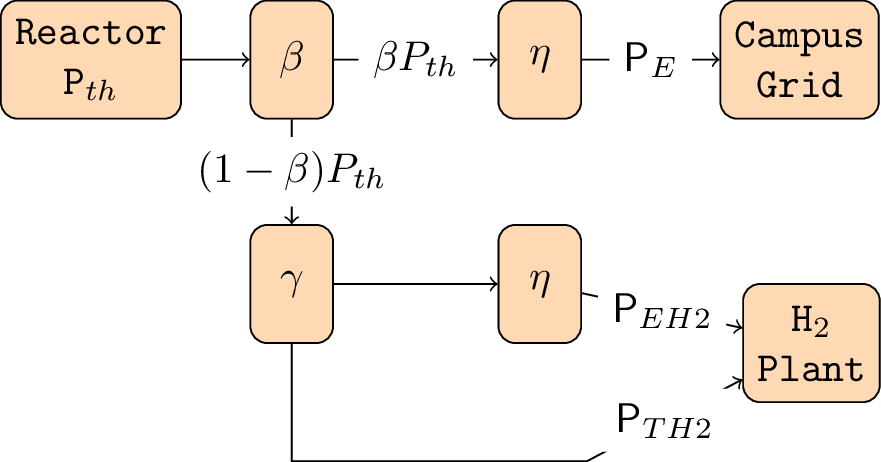
\includegraphics[height=4.5cm]{figures-hydro /hte-figure0.png}
	\hfill
	\caption{Diagram of a reactor coupled to a hydrogen plant.}
	\label{fig:cogen}
\end{figure}

\begin{align}
	P_{E} &= \eta \beta P_{th} 	\label{eq:cogen1} \\
	P_{EH2} &= \eta \gamma (1-\beta) P_{th} \\
	% \label{eq:cogen2}
	P_{TH2} &= (1-\gamma) (1-\beta) P_{th}
	\label{eq:cogen3}
	%\label{eq:cogen3}
	\intertext{where}
    \eta &= \mbox{thermal-to-electric conversion efficiency} \\
	% \label{eq:cogen4}
	\beta &= \frac{P_{E} / \eta}{P_{E} / \eta + P_{TH2}/(1-\gamma)} \\
	% \label{eq:cogen5}
	\gamma &= \frac{P_{EH2} / \eta}{P_{EH2} / \eta + P_{TH2}}.
	\label{eq:cogen6}
\end{align}

If $\beta = 1$, the reactor only supplies the grid with electricity $P_E$, and the hydrogen plant does not produce \gls{H2}.
If $\beta = 0$, the reactor only supplies the hydrogen plant, and no electricity goes into the grid.
Table \ref{tab:cogen1} summarizes the values that $\gamma$ takes for the different methods.

\begin{table}[htbp!]
    \centering
    \begin{tabular}{l|ccc}
        \hline
        Method    & $\gamma$         & $P_{EH2}$ & $P_{TH2}$ \\ \hline
        \gls{LTE} & 1                & $\ne$ 0   & 0         \\
        \gls{HTE} & $0 < \gamma < 1$ & $\ne$ 0   & $\ne$ 0   \\
        \gls{SI}  & 0                & 0         & $\ne$ 0   \\ \hline
    \end{tabular}
    \caption{Energy requirements of the different methods.}
    \label{tab:cogen1}
\end{table}

\section{Results}
\label{sec:Results}

This section holds the results of the different analyses.

\subsection{Transportation}

This subsection centers its focus on the transportation sector.
Figure \ref{fig:fuel} displays the fuel consumed per day by \gls{MTD} and \gls{UIUC} fleet.
Using the values shown in Table \ref{tab:equiv}, we calculate the \gls{H2} requirement for MTD and UIUC fleets, Figure \ref{fig:hydro-fleet}.
Table \ref{tab:hydro-fleet} summarizes the most important results.

	\begin{figure}[htbp!]
		\centering
		\begin{subfigure}[t]{0.4\textwidth}
			\centering
			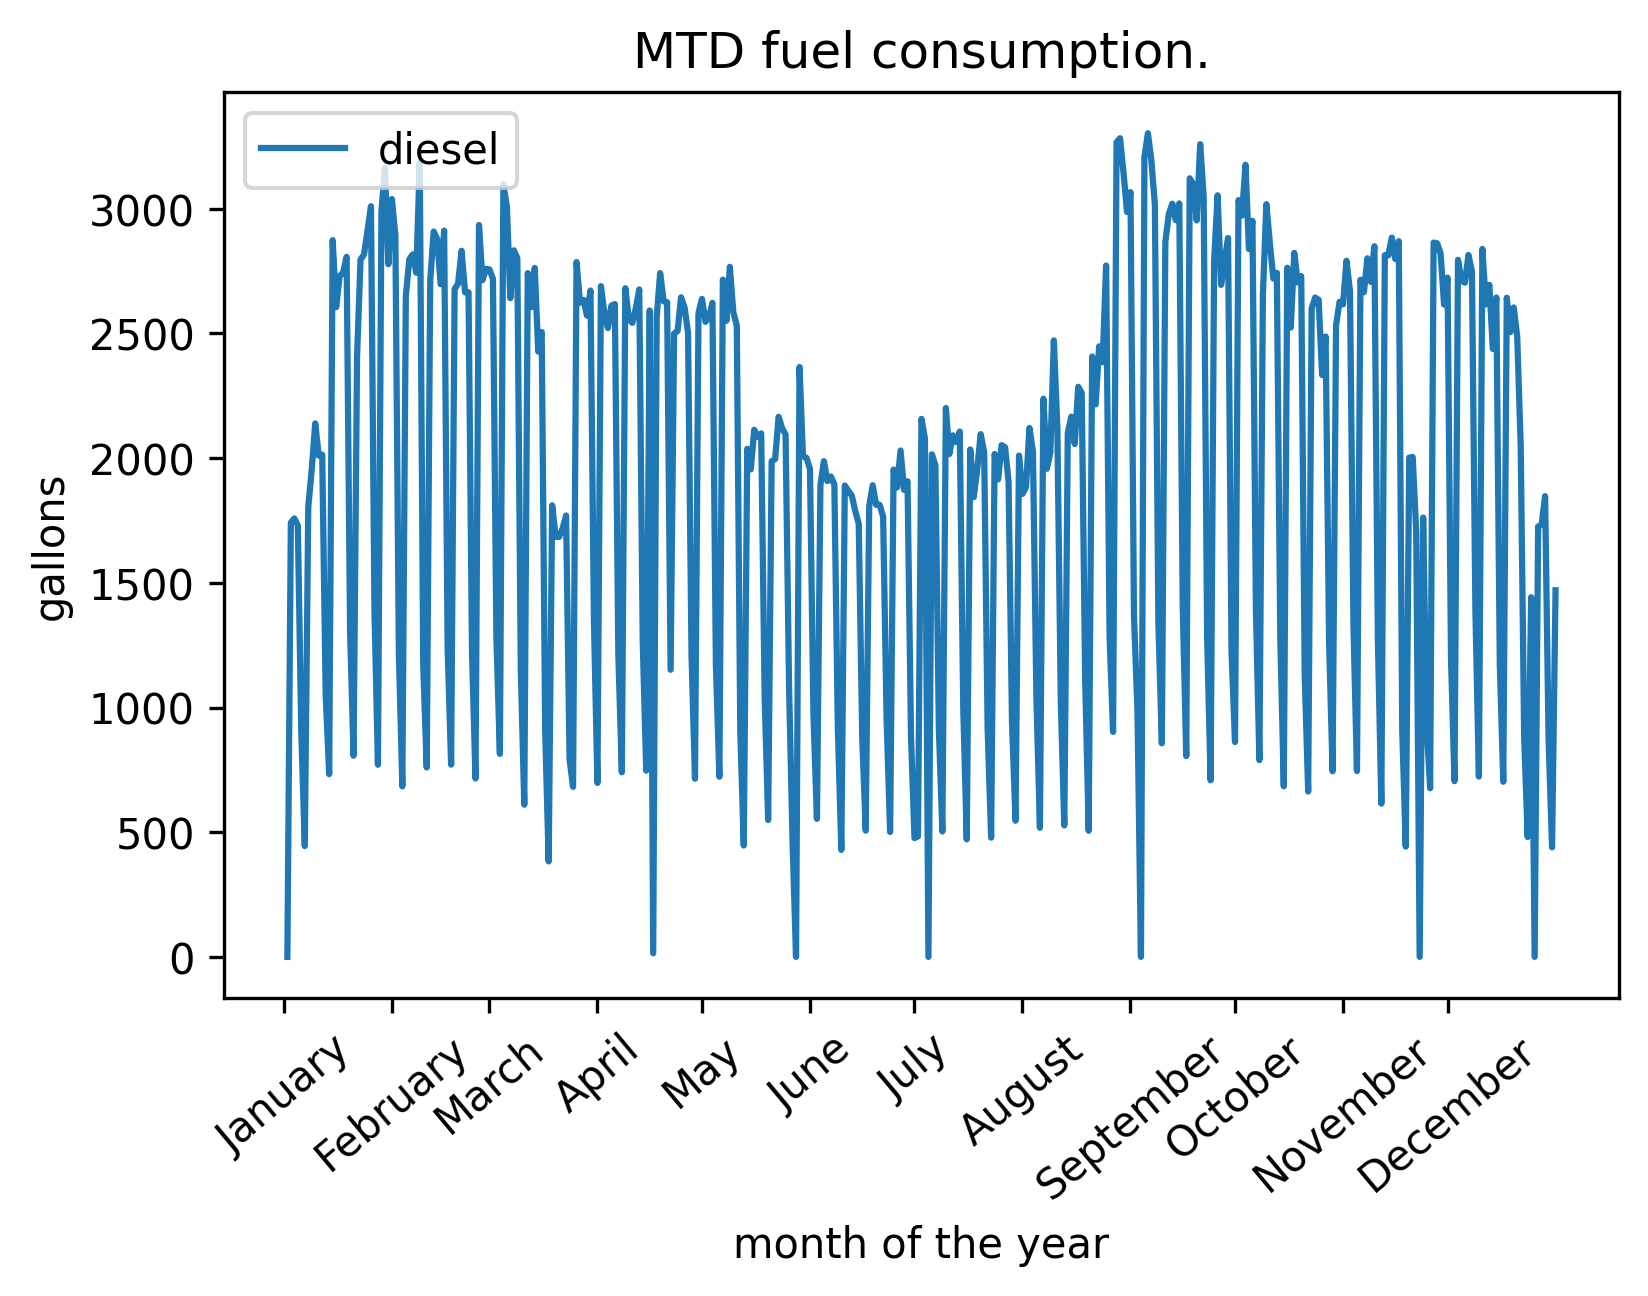
\includegraphics[width=\linewidth]{figures-hydro /mtd2}
			\caption{\gls{MTD} fleet. Data go from July 1, 2018, until June 30, 2019 \cite{mtd_irecords_2019}.}
		\end{subfigure}
		\begin{subfigure}[t]{0.4\textwidth}
			\centering
			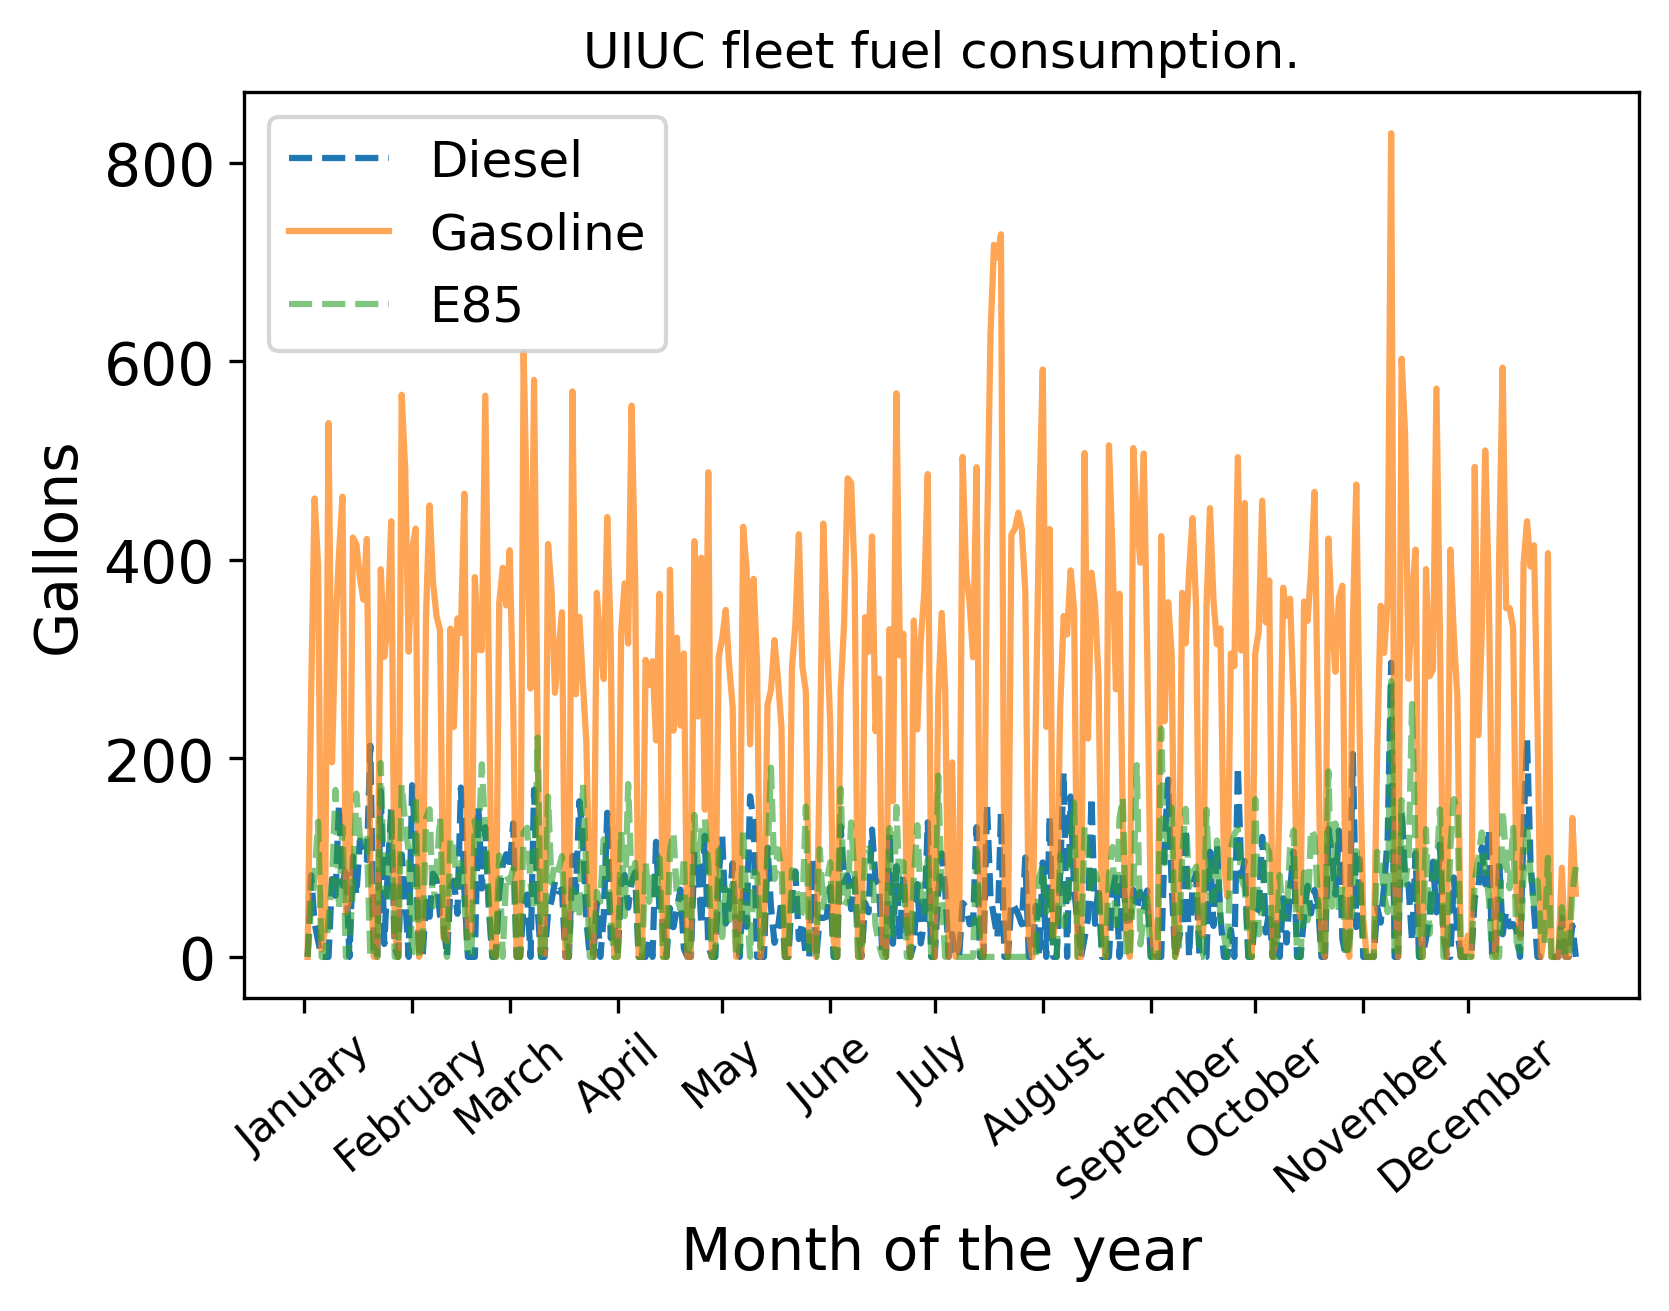
\includegraphics[width=\linewidth]{figures-hydro /uiuc}
			\caption{\gls{UIUC} fleet. Data go from January 1, 2019, until December 31, 2019 \cite{uiuc_personnal_communication}.}
		\end{subfigure}
		\hfill
		\caption{Fuel consumption data.}
		\label{fig:fuel}
	\end{figure}

	\begin{table}[htbp!]
	\centering
	\caption{\gls{H2} necessary to replace a gallon of fuel \cite{doe_office_of_energy_efficiency_and_renewable_energy_hydrogen_2020} \cite{alternative_fuels_data_center_fuel_2014}.}
	\begin{tabular}{l|c}
	    \hline
	 	                 & Hydrogen Mass [kg] \\ \hline
	 	Gasoline         & 1                  \\
	 	Diesel           & 1.13               \\
	 	E85              & 0.78               \\ \hline
	\end{tabular}
	\label{tab:equiv}
	\end{table}

	\begin{figure}[htbp!]
	    \centering
		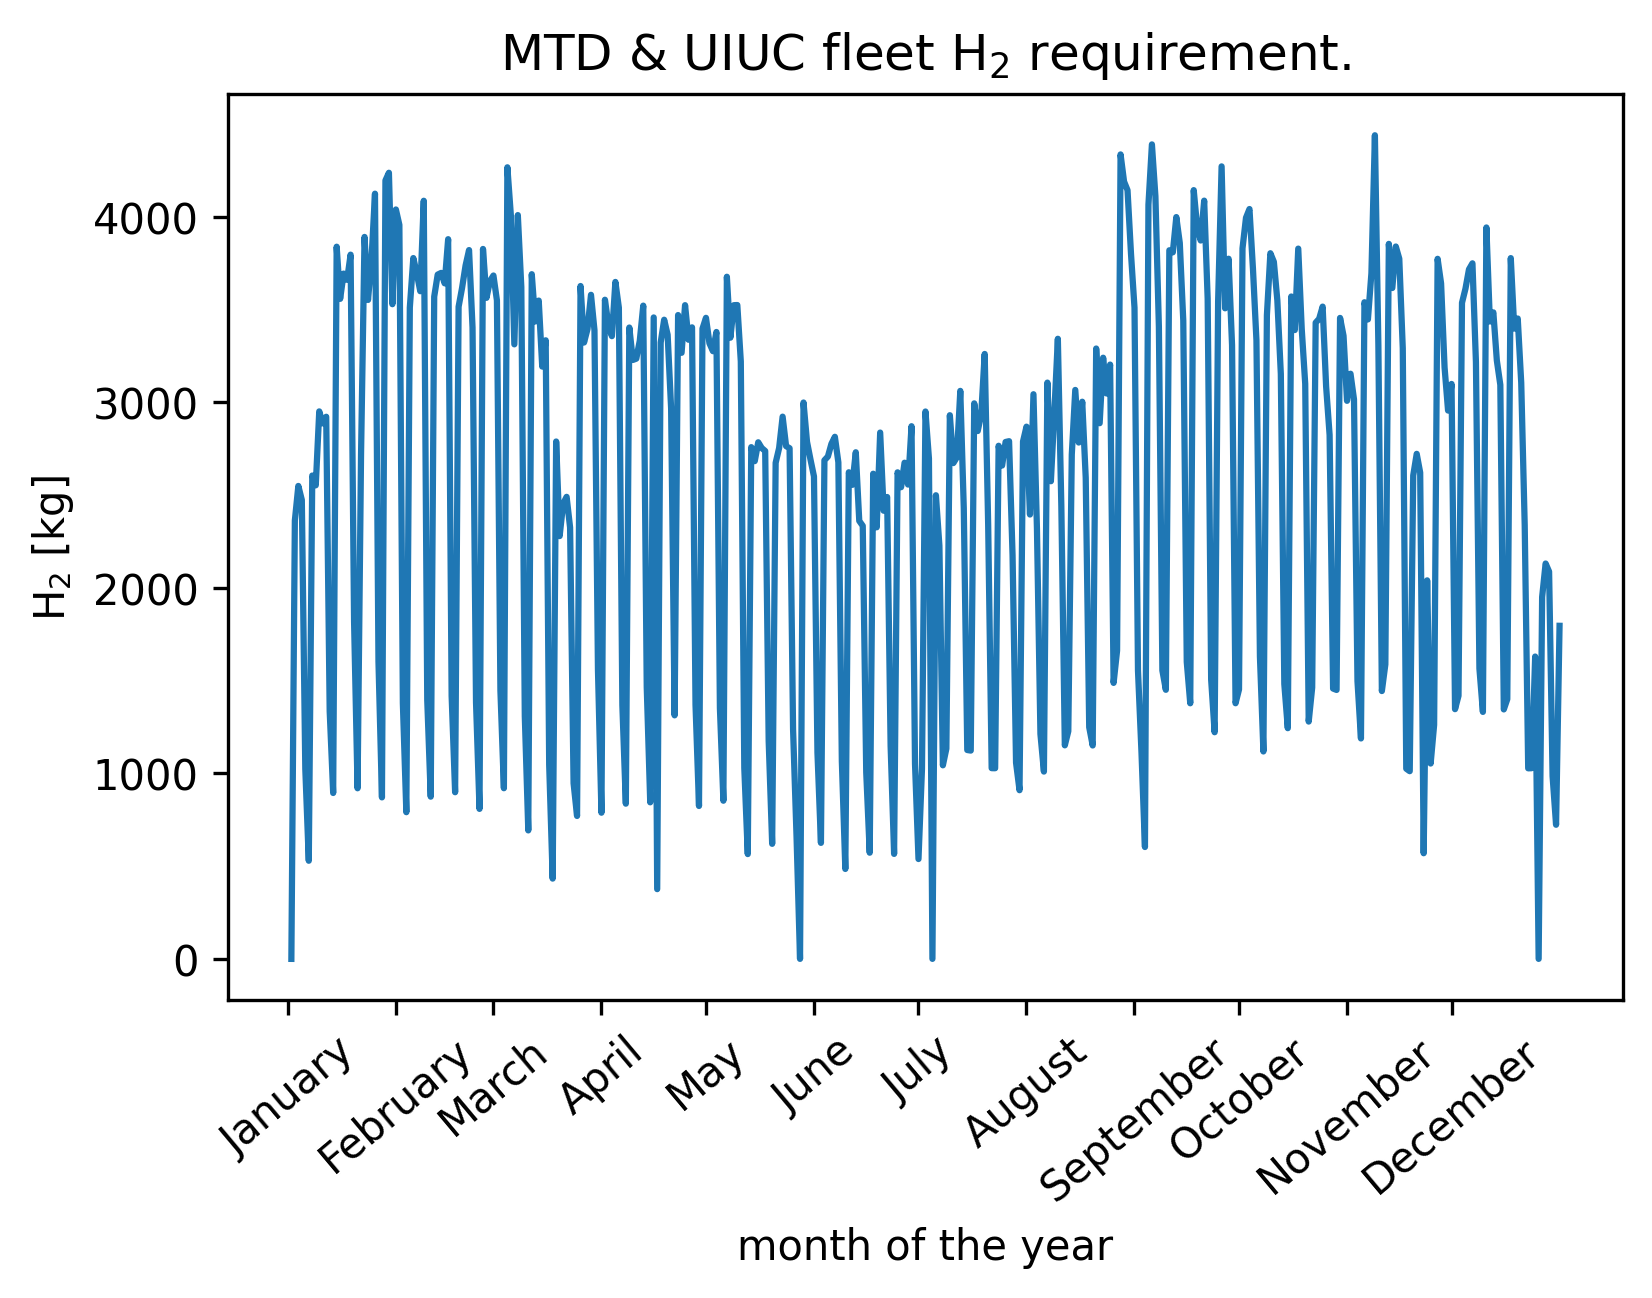
\includegraphics[height=7.0cm]{figures-hydro /hydro-fleet}
		\hfill
		\caption{\gls{H2} requirement for MTD and UIUC fleets.}
		\label{fig:hydro-fleet}
	\end{figure}

	\begin{table}[htbp!]
		\centering
	    \caption{\gls{H2} requirement for MTD and UIUC fleets.}
		\begin{tabular}{l|c}
		\hline
		Total [tonnes/year]     & 943    \\
		Average [kg/day] 	    & 2584   \\
		Average [kg/h] 		    & 108    \\
		Maximum in one day [kg] & 4440   \\ \hline
        \end{tabular}
        \label{tab:hydro-fleet}
	\end{table}

Using Table \ref{tab:co2-eq}, we calculate the \gls{CO2} savings caused by replacing all the fossil fuels by \gls{H2}.
Table \ref{tab:co2} displays the \gls{CO2} savings for both fleets.

	\begin{table}[htbp!]
		\centering
	    \caption{\gls{CO2} savings in lbs per gallon of fuel burned \cite{energy_information_administration_how_2014}.}
		\begin{tabular}{l|c}
		\hline
		              & \gls{CO2} produced [lbs/gallon] \\ \hline
		Gasoline      & 19.64           \\
		Diesel        & 22.38           \\
		E85           & 13.76           \\ \hline
        \end{tabular}
        \label{tab:co2-eq}
	\end{table}

	\begin{table}[htbp!]
		\centering
	    \caption{\gls{CO2} yearly savings.}
		\begin{tabular}{l|c}
		\hline
		            & \gls{CO2} mass [tonnes/year] \\ \hline
		MTD      	  & 7306           \\
		UIUC        & 1143           \\
		Total       & 8449           \\ \hline
        \end{tabular}
        \label{tab:co2}
	\end{table}

We have determined the \gls{H2} requirement by the fleets, and now we seek a microreactor design capable of meeting such demand.
For our analysis, we chose a few microreactor designs summarized in Table \ref{tab:hydro-micro}.
Further studies could include other designs as well.

Figure \ref{fig:hydro-micro} shows the hourly production rates for the different reactors and the \gls{H2} production processes.
The figure includes a continuous line that represents the hydrogen requirement of both fleets.
Note that the \gls{SI} process' required high temperatures allow for the coupling with only one microreactor design, which has an outlet temperature of more than 800$^{\circ}$C.

	\begin{table}[htbp!]
		\centering
	    \caption{Microreactor designs.}
		\begin{tabular}{l|cc}
		\hline
		Reactor                                      & P[MWt] & T$_o$[$^\circ$C] \\ \hline
		MMR \cite{usnc_mmr_2019}  		             & 15           & 640              \\
		eVinci \cite{hernandez_micro_2019}           & 5            & 650              \\
		ST-OTTO \cite{harlan_x-energy_2018}          & 30           & 750              \\
		U-battery \cite{ding_design_2011}            & 10           & 750              \\
		Starcore \cite{star_core_nuclear_star_2015}  & 36           & 850              \\ \hline
        \end{tabular}
        \label{tab:hydro-micro}
	\end{table}

	\begin{figure}[htbp!]
	    \centering
		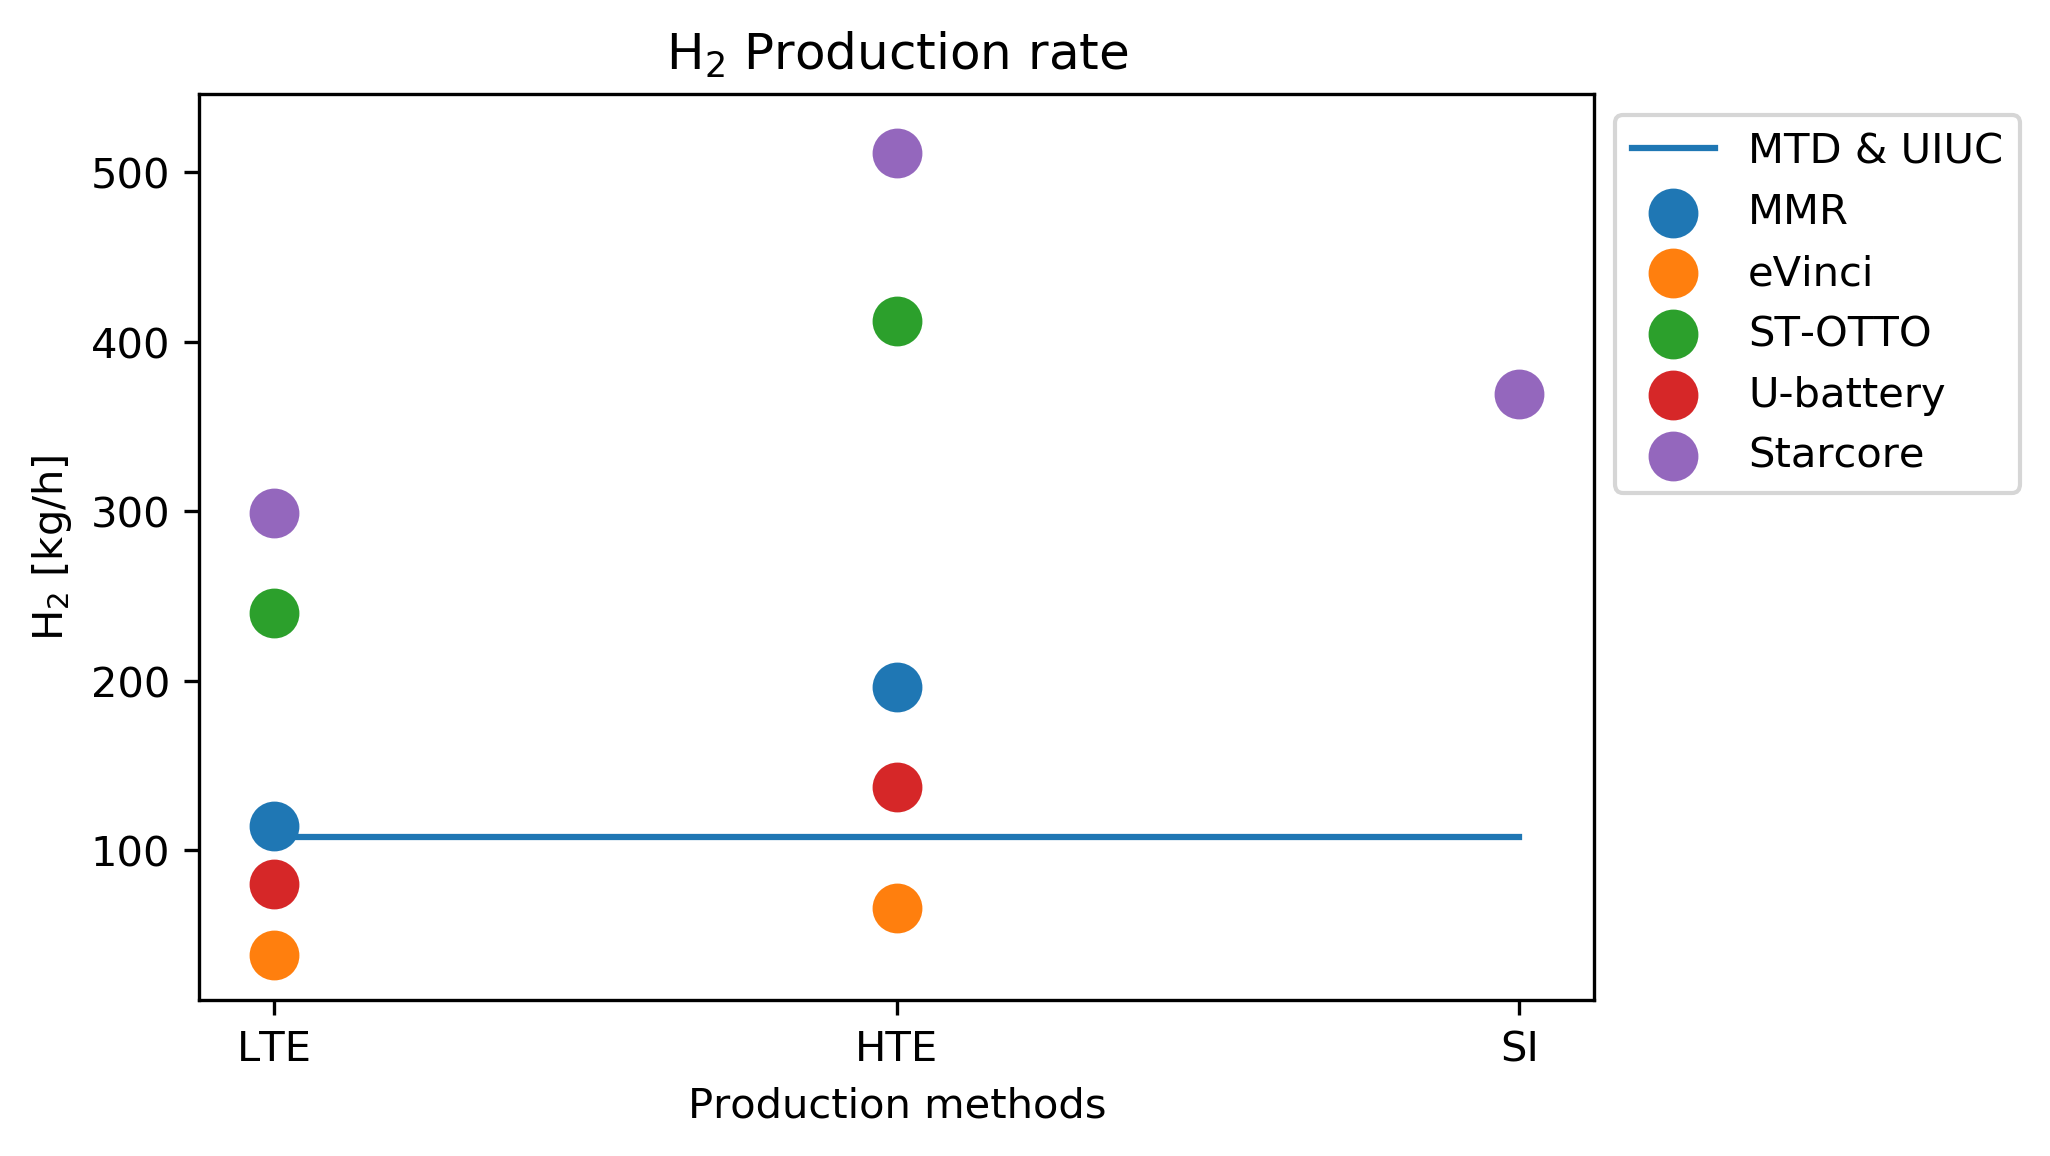
\includegraphics[height=6.0cm]{figures-hydro /reactors-by-hour1}
		\hfill
		\caption{Hydrogen production rate by the different microreactor designs.}
		\label{fig:hydro-micro}
	\end{figure}

\subsection{Electricity Generation}

This subsection centers its focus on the electricity generation sector and the duck curve problem.
To quantify the duck curve's magnitude, we have to predict the \gls{UIUC} grid's load and the expected electricity production from solar. 
As the \gls{icap}'s main objective is to become carbon neutral before 2050, we make our prediction for that year.
\gls{UIUC} solar farm is relatively new, and the data available is not enough for producing a reliable forecast.
To go around this barrier, we use the available data for the whole \gls{US}.
Figure \ref{fig:prediction} displays the prediction for 2050.
We carry out the prediction using a linear regression that produces the worst-case scenario.
In such a scenario, the total load does not increase considerably, whereas the solar generation does.

\begin{figure}[htbp!]
	\centering
	\begin{subfigure}[t]{0.38\textwidth}
		\centering
		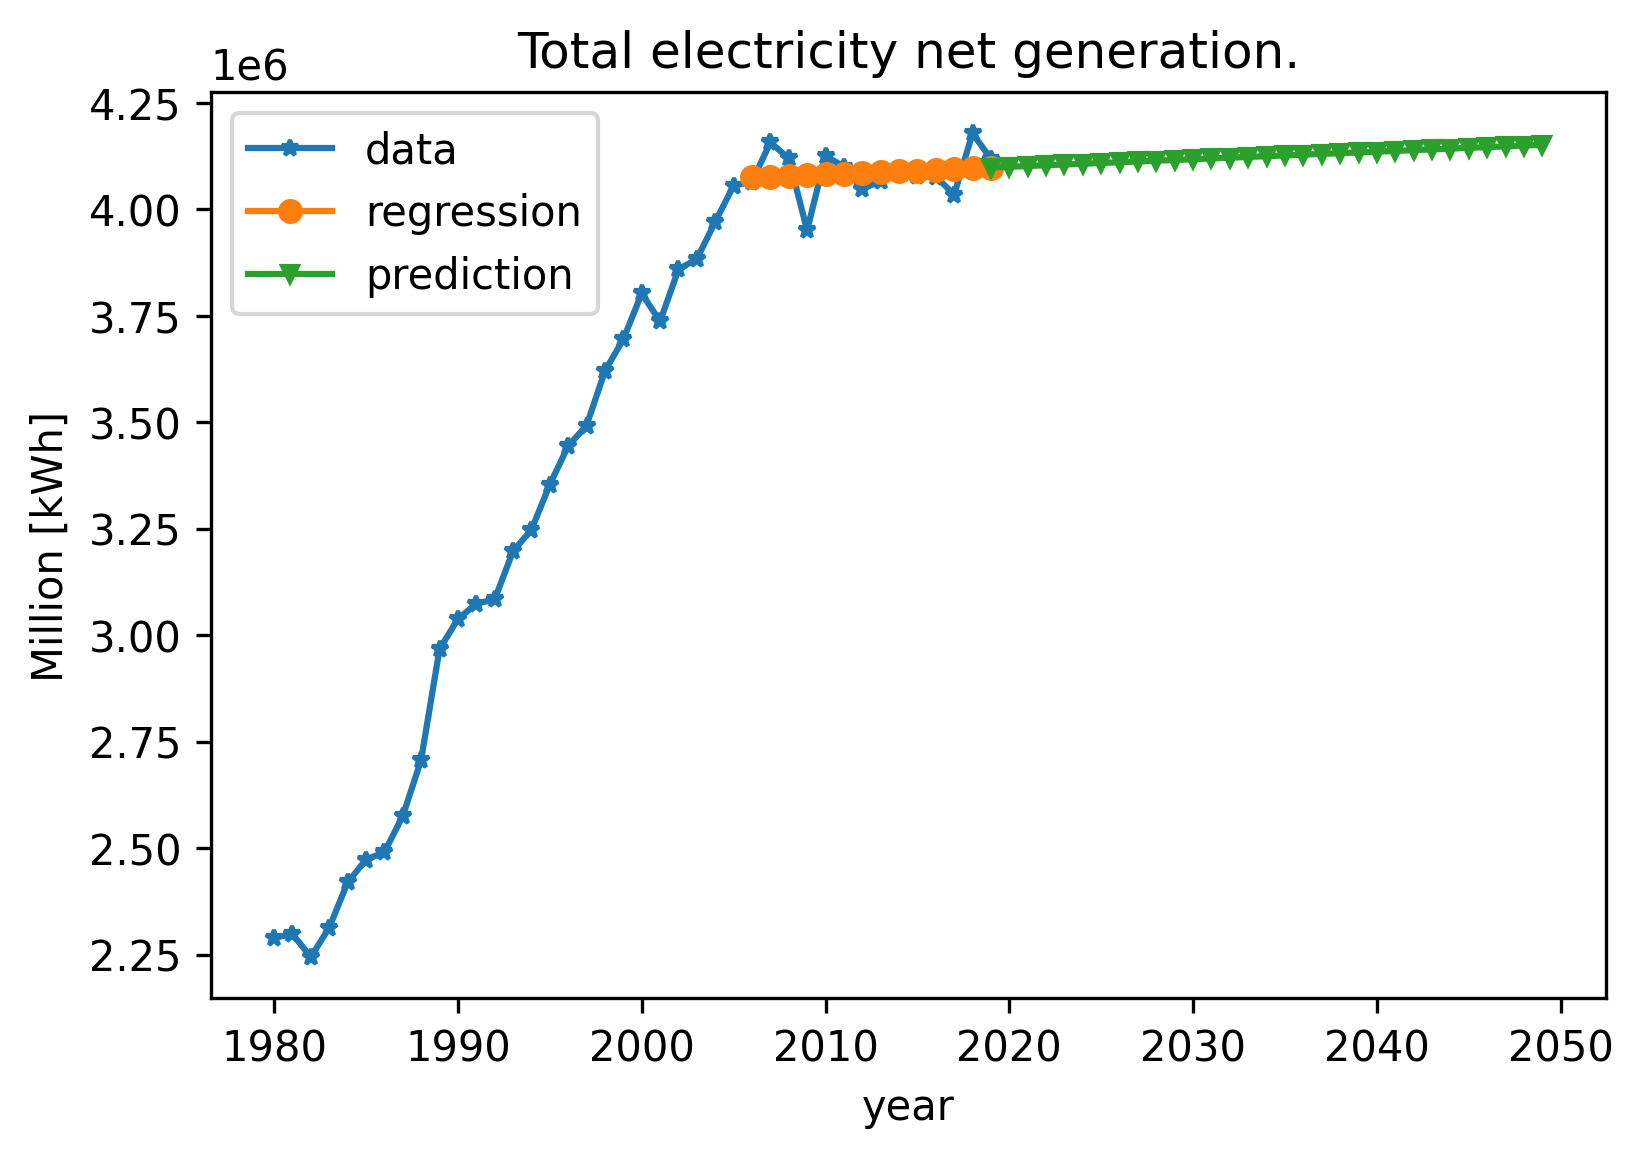
\includegraphics[width=\linewidth]{figures-hydro /us-prediction1}
		\caption{Total electricity generation.}
	\end{subfigure}
	\begin{subfigure}[t]{0.40\textwidth}
		\centering
		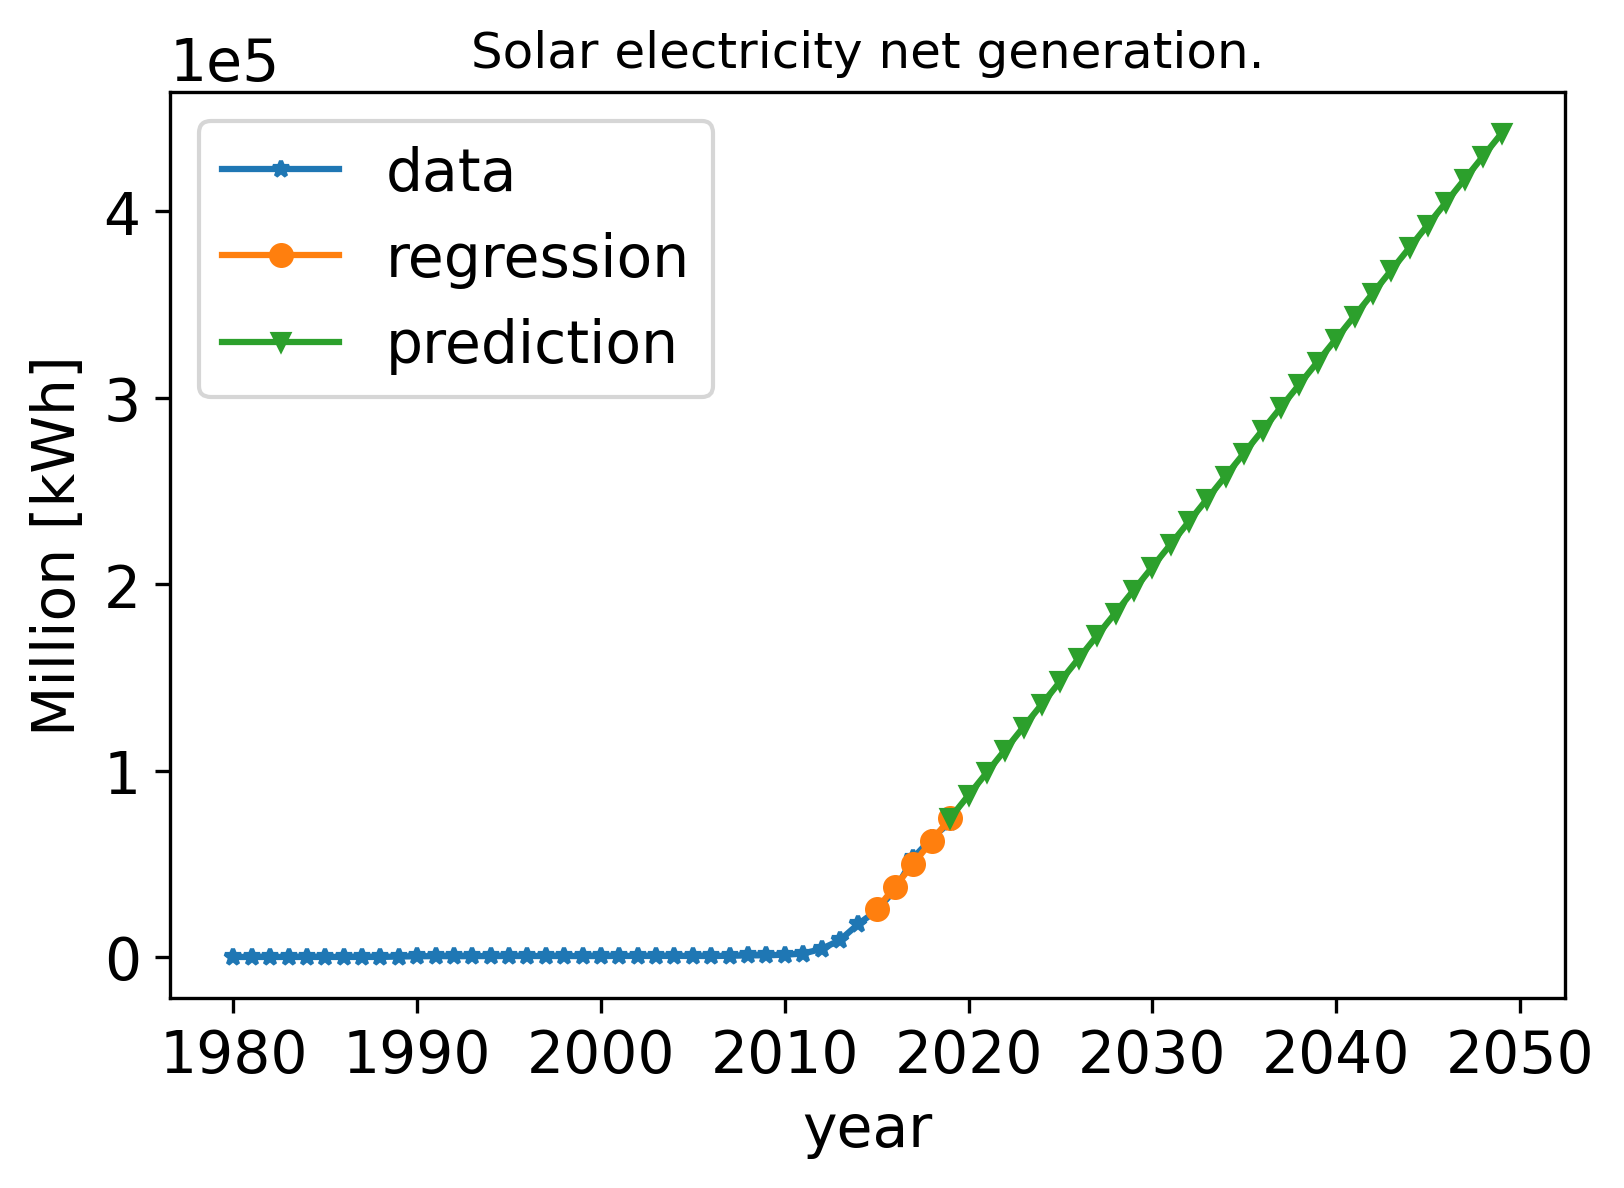
\includegraphics[width=\linewidth]{figures-hydro /us-prediction2}
		\caption{Solar electricity generation.}
	\end{subfigure}
	\hfill
	\caption{Prediction of the electricity generation in the \gls{US} for 2050. Data from \cite{us_energy_information_administration_electric_2020}.}
	\label{fig:prediction}
\end{figure}

The next step was to apply the same growth factor from the predictions to the \gls{UIUC} grid's load and solar electricity.
To obtain a prediction for 2050, we apply the growth factor to the hourly data.
We choose a spring day when solar production is higher, as it is sunny, but the total load is low since people are not using electricity for air conditioning or heating \cite{us_department_of_energy_confronting_2017}.
Finally, we subtract the solar production from the total load, obtaining the net load or demand ($D_{NET}$).

We narrowed our analysis' focus to April 4th, when the net demand reached the lowest value in the 2019's spring.
Figure \ref{fig:uiuc-duck1} shows these results.
In 2050, the peak net demand will be 46.9 MWh at 5 PM.
The lowest net demand will be 15 MWh at 11 AM.
These results yield a demand ramp of 31.9 MWh in 4 hours.
These results show that the grid requires an available capacity of dispatchable sources of at least 31.9 MW.

\begin{figure}[htbp!]
		\centering
	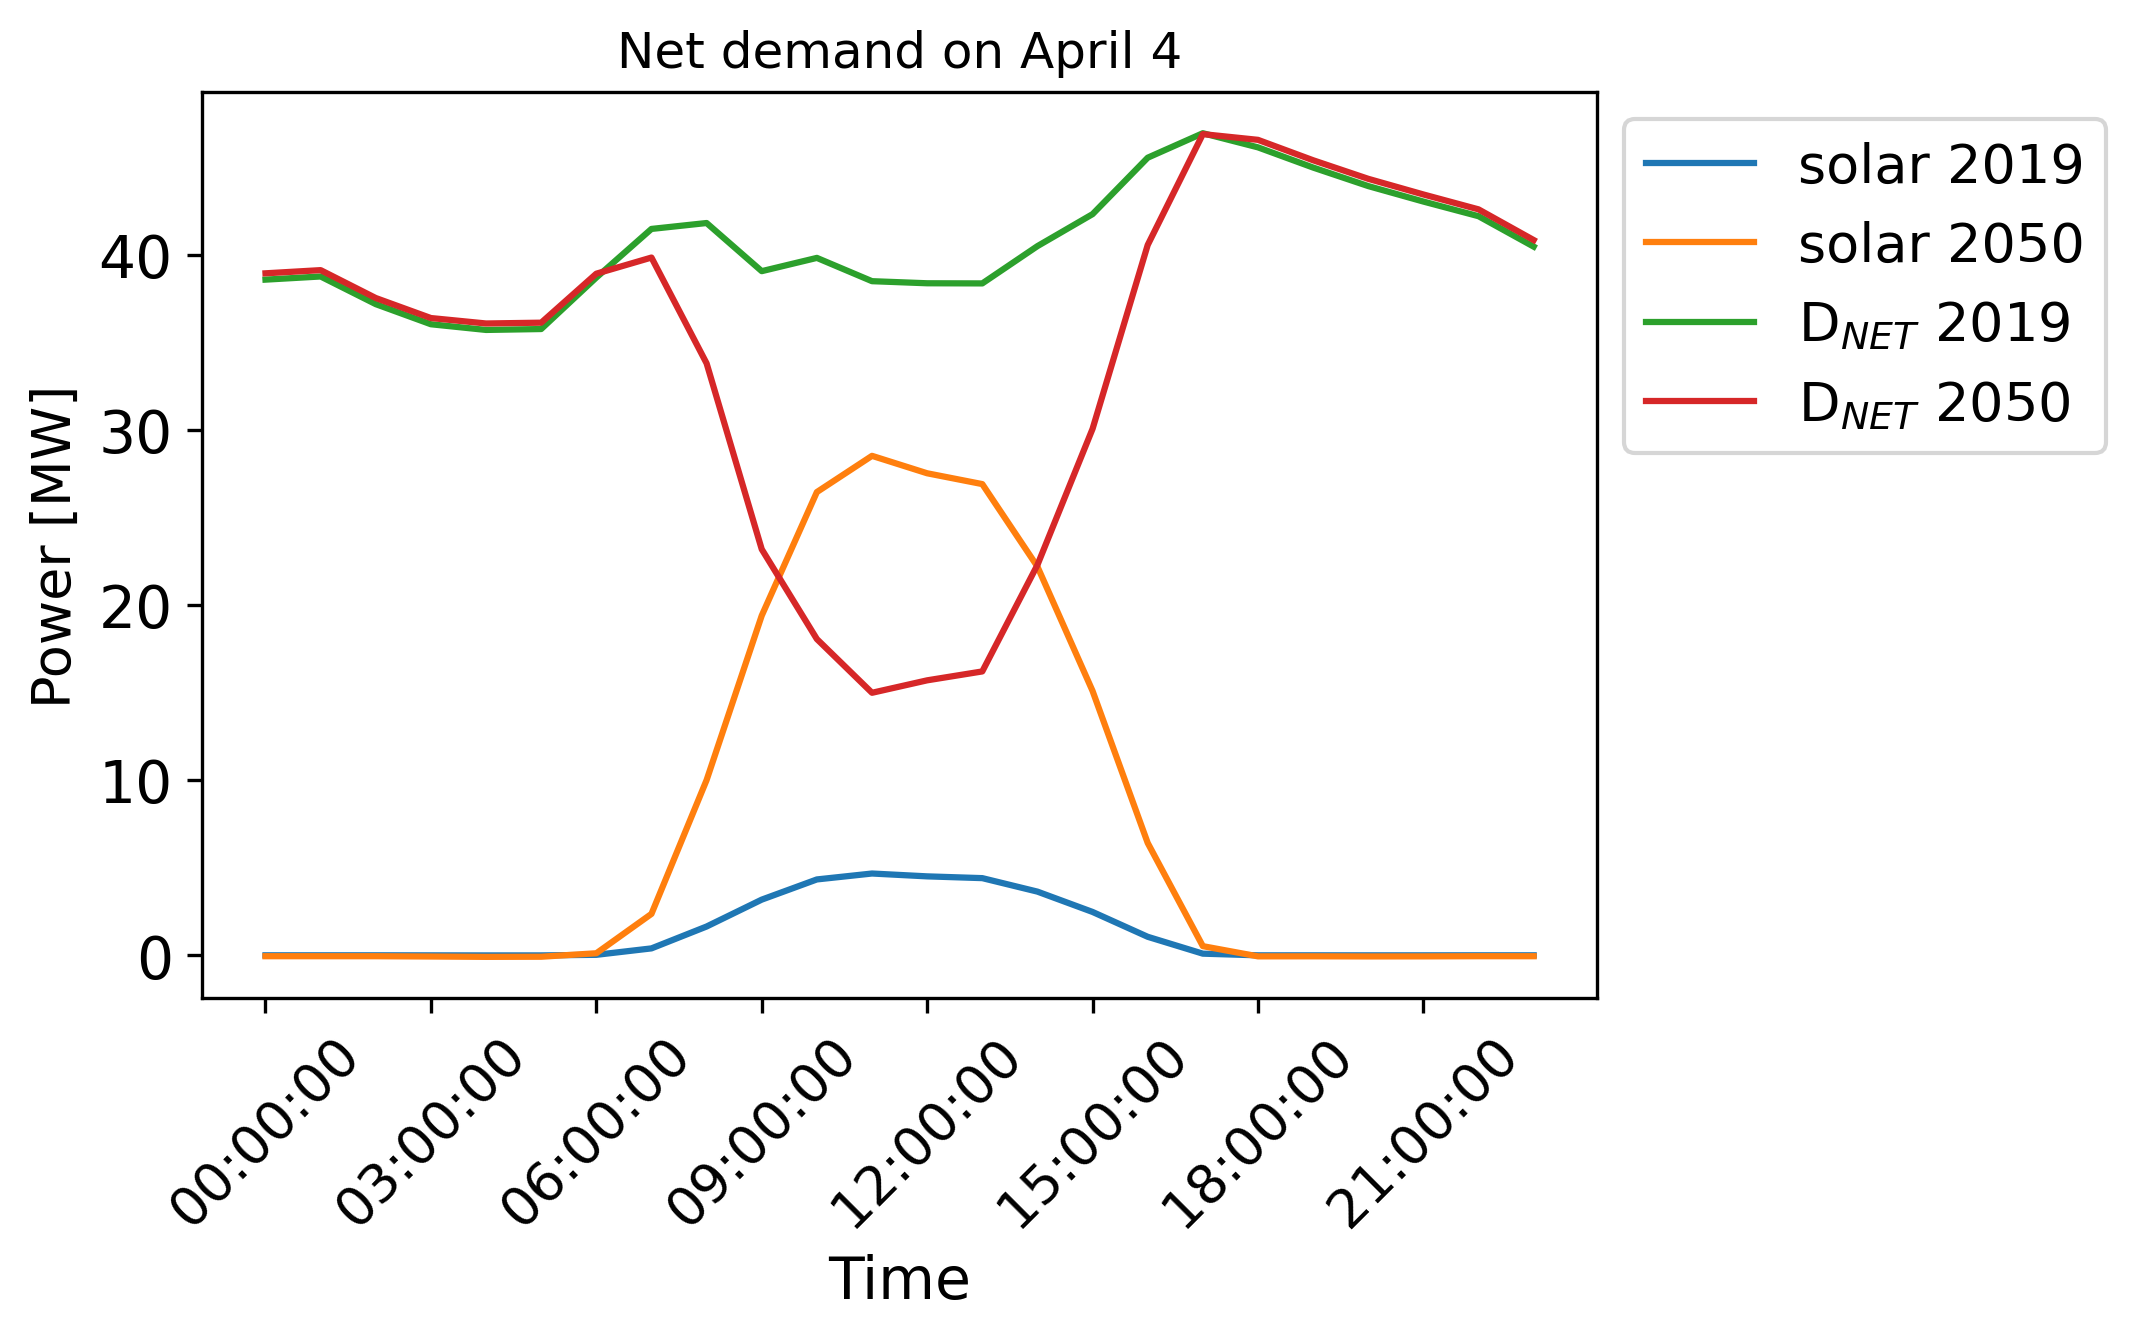
\includegraphics[height=5cm]{figures-hydro /uiuc-duck}
	\hfill
	\caption{Prediction of \gls{UIUC}'s net demand for 2050.}
	\label{fig:uiuc-duck1}
\end{figure}

% Big part of this should go in the methodology section
Once we calculated the net demand, the next step was to figure the over-generated electricity.
For that purpose, we arbitrarily chose a reactor of 25 MW.
For the \gls{LTE} case, any reactor is a valid option.
We chose an $\eta$ of 33$\%$, which yields a reactor power of 75.8 MWt.
For the \gls{HTE} case, the reactor's choice is an HTGR with an outlet temperature of 850$^{\circ}$C.
We consider an $\eta$ of 49.8$\%$, which yields a reactor of 50.2 MWt.

The reactor operates at full capacity at all times.
However, the reactor electricity ($P_{E}$) equals the net demand ($D_{NET}$) once smaller than 25 MW.
Note that $P_{E}$ has power units while $D_{NET}$ has energy units.
We chose time steps of 1 hour for our analysis, hence $P_{E}$ and $D_{NET}$ differ by the constant $h$.
As $P_{E}$ is lower than 25 MW, and the reactor is at full thermal capacity, the hydrogen plant takes the excess of thermal energy.
We use equation \ref{eq:demand} with equations \ref{eq:cogen1} to \ref{eq:cogen6} to calculate the hydrogen produced.
Figure \ref{fig:uiuc-duck2} displays the results.
The total \gls{H2} production reaches 660, 1009, and 815 kg for \gls{LTE}, \gls{HTE}, and \gls{SI}.

\begin{align}
	P_{E} &= D_{NET}  \notag \\
  \frac{P_{E}}{25 MW} &= \frac{\eta \beta P_{th}}{\eta P_{th}} = \beta  \label{eq:demand}
\end{align}

% \begin{align}
	% P_{E} &= $D_{NET}$  \notag \\
  % \frac{P_{E}}{25 MW} &= \frac{\eta \beta P_{th}}{\eta P_{th}} = \beta  \label{eq:demand}
% \end{align}

\begin{figure}[htbp!]
		\centering
	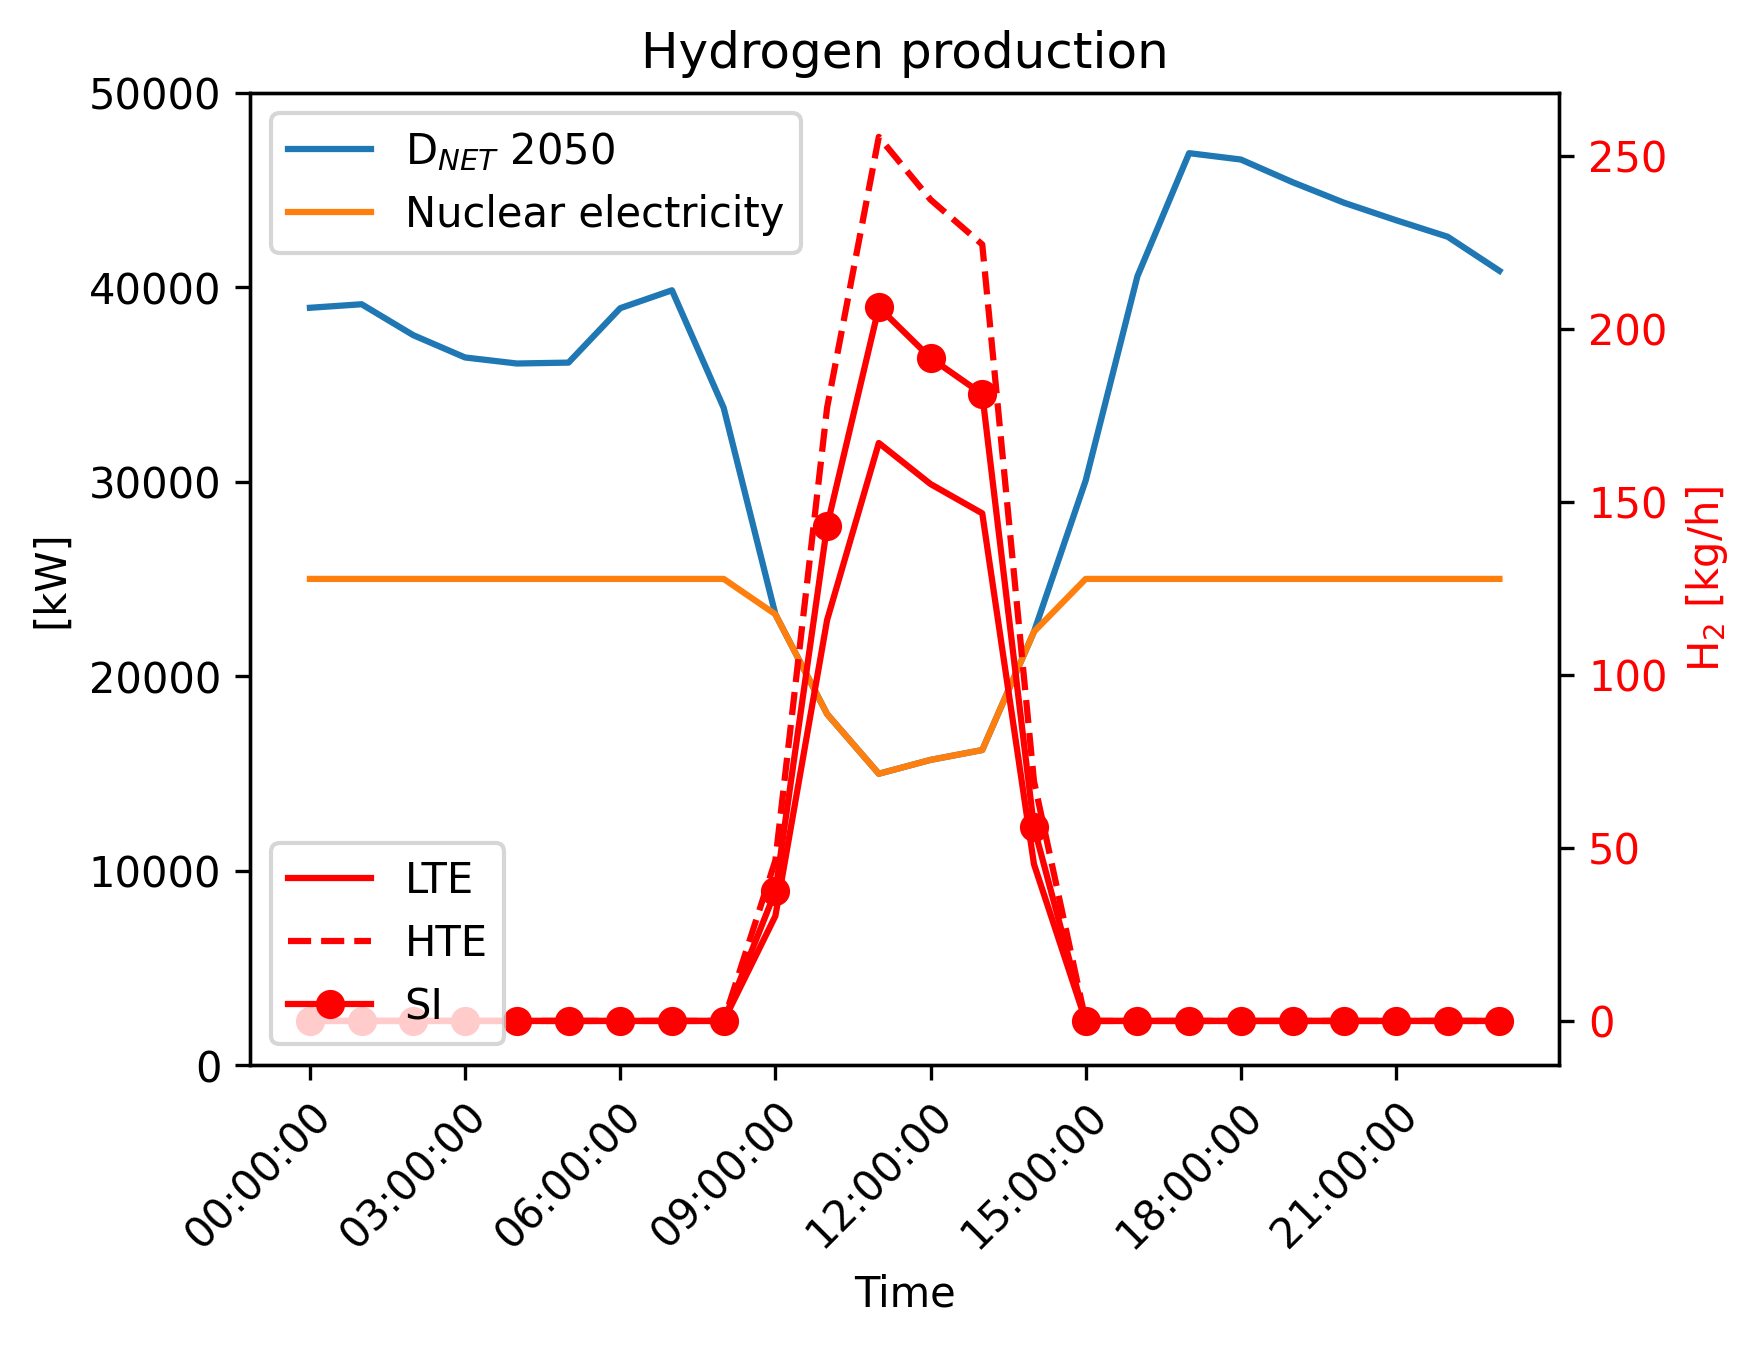
\includegraphics[height=5cm]{figures-hydro /uiuc-hydro2B}
	\hfill
	\caption{\gls{H2} production.}
	\label{fig:uiuc-duck2}
\end{figure}

% This should definitely be in Methodology
Our analysis last step is to calculate the peak demand reduction by using the hydrogen to produce electricity.
The energy produced by hydrogen is $285 kJ/mol$, equal to 40 kWh/kg \cite{ursua_hydrogen_2012}.
However, conventional fuel cells can use up to 60$\%$ of that energy \cite{doe_energy_efficiency_and_renewable_energy_fuel_2015}.
Knowing the mass of hydrogen produced, we calculate the total electricity produced.
We now reduce the peak demand by distributing the electricity over a specific range of hours.
We chose to distribute the electricity for over 6 hours.
We calculate the new peak using equation \ref{eq:newpeak}.
Figure \ref{fig:uiuc-duck3} shows these results.
The different \gls{H2} processes can generate 15.84 MWh, 24.2 MWh, and 19.6 MWh, respectively.
This generation accounts for a peak reduction of 5 MW, 6.4 MW, and 5.6 MW, respectively.

\begin{align}
	NP &= \frac{\sum_{i=0}^{N} D_{NET, i} - TH}{N} \\
	\label{eq:newpeak}
	\intertext{where}
		NP &= \mbox{New peak magnitude} \\
		D_{NET, i} &= \mbox{Hourly net demant} \\
		TH &= \mbox{Total mass oh hydrogen} \\
		N &= \mbox{Total number of hours when we use the \gls{H2}}
\end{align}

\begin{figure}[htbp!]
    \centering
	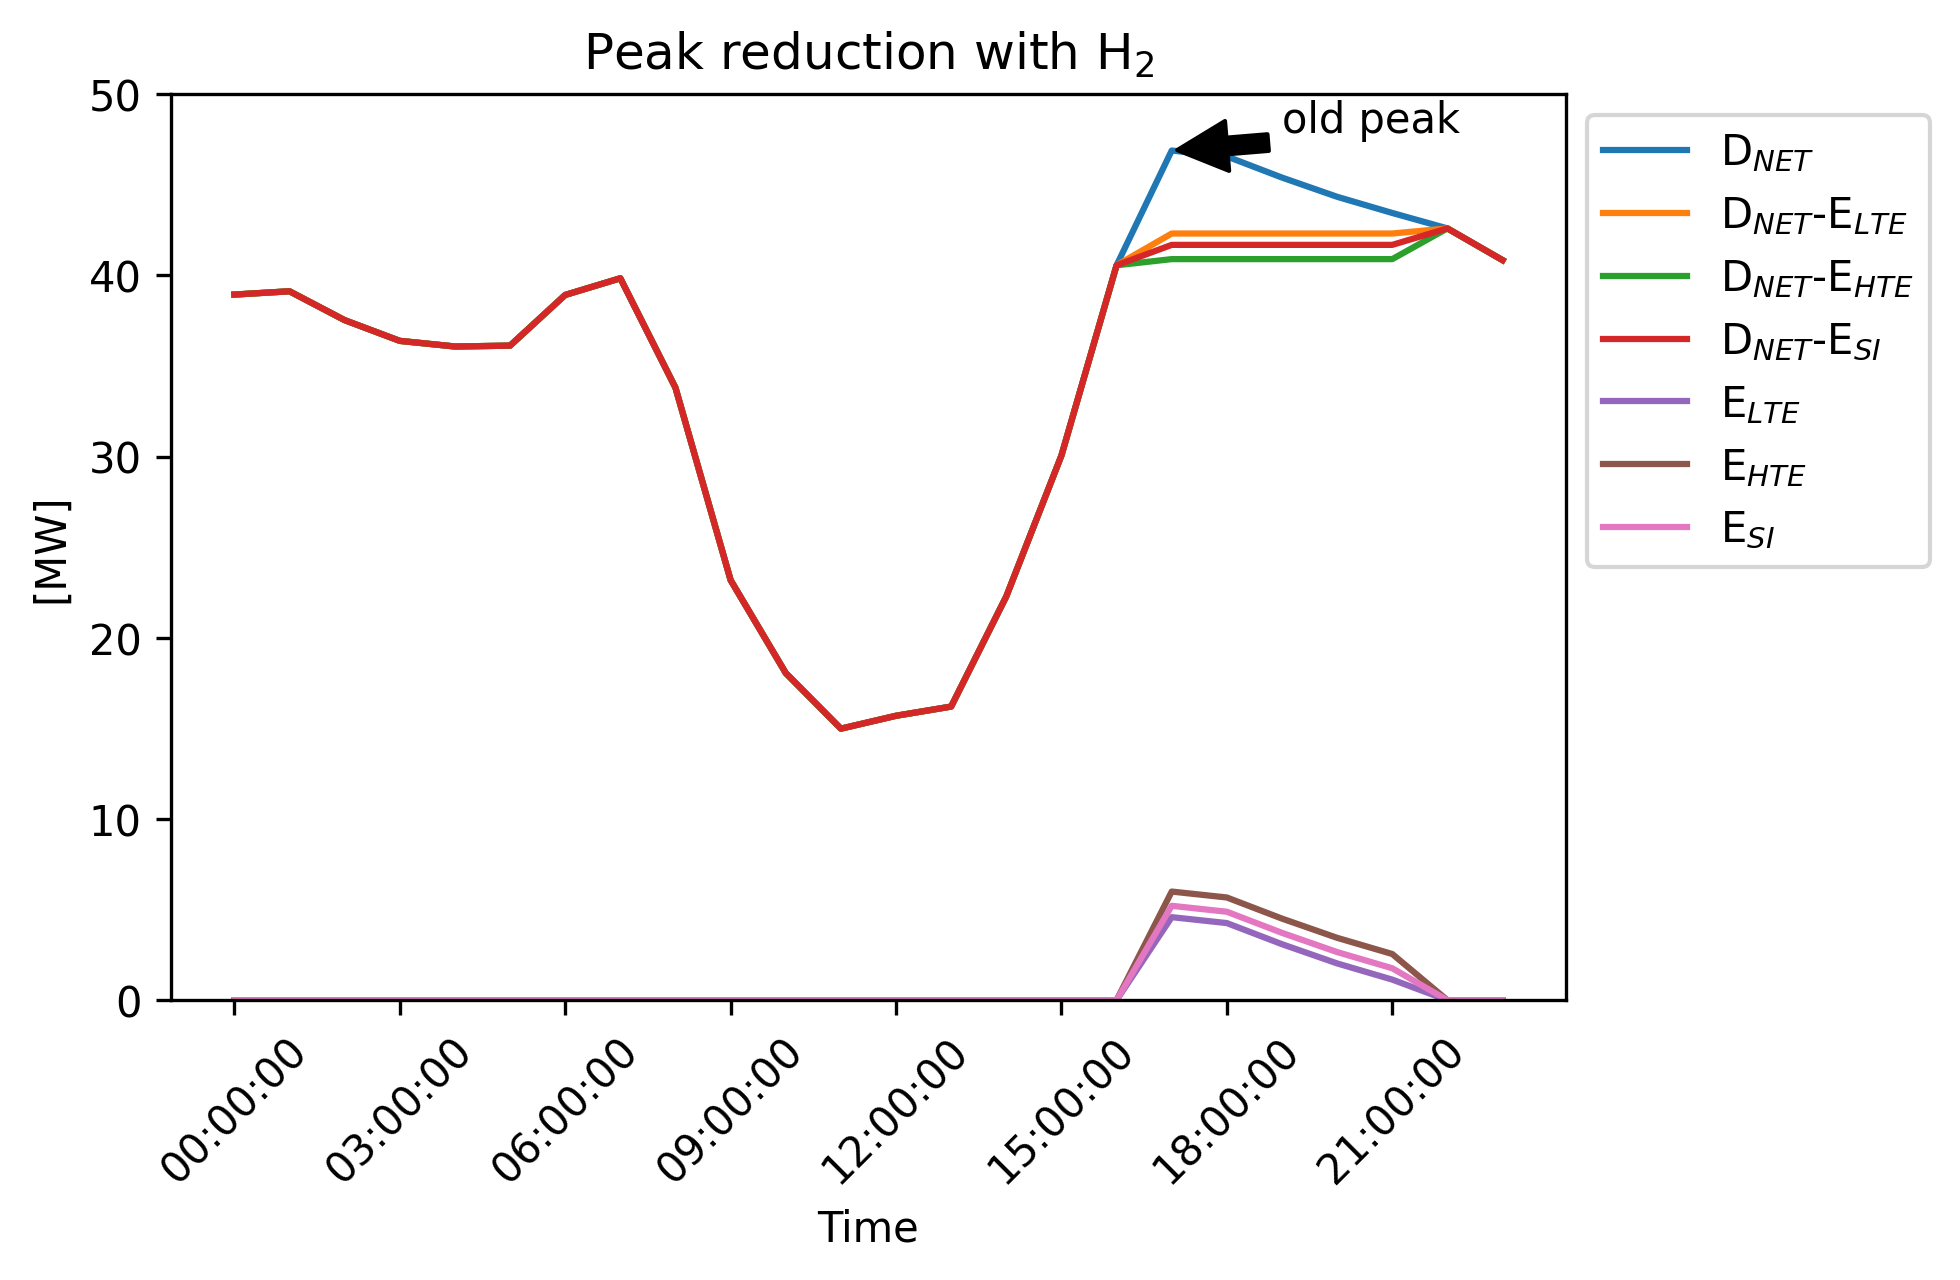
\includegraphics[height=5cm]{figures-hydro /uiuc-hydro3}
	\hfill
	\caption{Peak reduction by using the produced H$_2$.}
	\label{fig:uiuc-duck3}
\end{figure}

\section{Conclusions}

The world faces energy challenges that compromise the efforts to stop climate change.
The electricity generation and transportation sectors are the largest issuers of \glspl{GHG} and, hence, the major contributors to climate change.
These challenges underscore the need for cleaner sources.
Nonetheless, the common belief that renewable energy is the solution to the problem presents several drawbacks.
The duck curve is an example of such drawbacks.
Moreover, a carbon-neutral electric grid will be insufficient to halt climate change.
The transportation sector needs to survey some possible alternatives to become carbon-free as well.
In this work, we proposed combining nuclear energy and hydrogen production that represents a possible solution to these challenges.

To seek a solution for the challenge described above, we narrowed down our focus on a more particular case, the University of Illinois.
Through the implementation of the \gls{icap}, the University of Illinois is actively working to reduce \gls{GHG} emissions on its campus.
This work's objective aligns with the efforts in two of the six target areas defined on the \gls{icap}, electricity generation, and transportation.

Regarding hydrogen production methods, we surveyed three different processes: \gls{LTE}, \gls{HTE}, and \gls{SI}.
We developed a tool to calculate their energy requirements, regarding electricity and heat, and hydrogen production rates.
This tool is applicable to a stand-alone hydrogen plant and a nuclear power plant that produces both electricity and hydrogen.

In the transportation sector analysis, we quantified the fuel requirements of \gls{MTD} and \gls{UIUC} fleets.
We calculated the mass of hydrogen necessary to replace 100$\%$ of the fleet's fossil fuel usage.
Finally, we chose several microreactor designs, and we calculated their hydrogen production rates.
The microreactors that can meet both fleet hydrogen needs are the MMR, ST-OTTO, U-battery, and Starcore.
Starcore design is the only one that could use the \gls{SI} process.

In the electricity generation sector analysis, we predicted the duck curves' magnitude in UIUC's grid in 2050.
This result exhibits how an increased solar penetration into the grid worsens the duck curve.
We proposed a mitigation strategy that uses a microreactor of 25 MWe.
For such a reactor, we calculated the mass of hydrogen produced by the different methods during the day.
Finally, we estimated a peak demand reduction by using the hydrogen produced during the day.
This last result highlights that hydrogen introduces a means to store energy that reduces the reliance on dispatchable sources.
This analysis emphasizes how nuclear energy and hydrogen production are an approach to mitigate climate change.

\pagebreak
\bibliographystyle{plain}
\bibliography{bibliography}

\end{document}
